\documentclass[a4paper, 12pt]{article}

% --- PACKAGES ---
\usepackage{ctex} % 确保UTF-8中文支持
\usepackage[left=2.5cm, right=2.5cm, top=2.5cm, bottom=2.5cm]{geometry}
\usepackage{amsmath, amssymb, amsthm}
\usepackage{graphicx} % 用于插入图片
\usepackage{hyperref}
\usepackage{enumitem}
%\usepackage{natbib}
% 将原来的 \usepackage{natbib} 改为：
%\usepackage[super,comma,sort&compress]{natbib}
\usepackage{algorithm}
\usepackage[noend]{algpseudocode}
\usepackage{caption}
% 需要导入的表格的包
\usepackage{booktabs}
\usepackage{multirow}
\usepackage{colortbl}
\usepackage{xcolor}
\usepackage{makecell}
\usepackage{graphicx}
\usepackage{amssymb}
\newtheorem{theorem}[Theorem]

\title{TMSKD: Temporal--Memory Structure-Aware Knowledge Distillation for BiTAL-based Underwater Acoustic Target Recognition}
% \author{}
\date{}   

% \renewcommand{\bibname}{参考文献}
\begin{document}
\maketitle
% -------- 摘要 --------
\begin{abstract}
深度学习已显著推动了水下声学目标识别（UATR）的发展，然而，在资源受限的水下平台上部署复杂的深度模型仍是一项巨大的挑战。知识蒸馏（KD）技术通过将知识从高性能的教师模型转移到轻量级的学生模型中，有效缓解了这一难题。
然而，现有的水下声学目标识别知识蒸馏方法往往忽视了声学信号固有的多尺度时序结构，从而限制了学生模型对复杂时序依赖关系的建模能力。
为了解决这一问题，本文提出了一种时序-记忆结构感知知识蒸馏（TMSKD）框架，并采用双向时序感知液态神经网络（Bidirectional Temporal-Aware Liquid Network, BiTAL）作为学生模型。BiTAL 提供强大的神经动力学建模能力，并集成了两种互补的蒸馏策略：一是自适应温度的时序分离（TS-T）蒸馏，用以提升逐时间步语义分布对齐能力；二是记忆差异知识蒸馏（MemKD），通过实施记忆感知对齐，以保留跨时间尺度下鲁棒的判别性信息。在两个真实海洋数据集上的广泛实验证实，TMSKD 相比现有的知识蒸馏方法展现出更优异的性能，在 ShipsEar 上实现了 92.39\% 的识别准确率（ACC），相比竞争性基线结果 90.03\% 提升了 2.36 个百分点。值得注意的是，TMSKD 使 BiTAL 学生模型的识别准确率显著提升了 4.14 个百分点。
% 水声目标识别（Underwater Acoustic Target Recognition, UATR）在深度学习技术的推动下取得了显著进展。然而，受限于水下平台有限的计算与存储资源，复杂深度模型在实际部署中仍面临较大挑战。知识蒸馏（Knowledge Distillation, KD）通过将高性能教师模型中的知识迁移至轻量化学生模型，为提升模型实用性提供了一种有效途径。然而，现有面向 UATR 的蒸馏方法往往忽视水声信号固有的多尺度时间结构特性，导致轻量模型在时序建模能力和识别性能方面存在不足。

% 针对上述问题，受生物神经元中自适应连续动力学启发，本文提出了一种采用双向时序感知液态神经网络（Bidirectional Temporal-Aware Liquid Network, BiTAL）的多时间结构感知知识蒸馏方法（Temporal–Memory Structure-Aware Knowledge Distillation, TMSKD），用于构建高效且精确的水声目标识别模型。本文选用预训练的 wav2vec 2.0 作为教师网络，以充分挖掘水声信号中的高层时序语义信息；同时，引入 BiTAL 作为学生网络，以满足神经元动态建模能力和低计算复杂度的需求。TMSKD融合了两种互补的蒸馏策略：时间语义增强表示蒸馏（Temporal Semantic Enhanced Representation Distillation, TSER） 与 基于记忆差异的知识蒸馏（Memory-Discrepancy Knowledge Distillation, MemKD）。其中，TSER 引导学生网络学习教师模型中具有判别力的时间语义结构，增强其对长时依赖关系的建模能力；MemKD 则通过记忆感知的特征对齐机制，在不同时间尺度上保留稳定且鲁棒的判别信息。

% 在真实海洋水声数据集上的大量实验结果表明，采用 BiTAL 的 TMSKD 方法在识别精度上显著优于现有知识蒸馏方法。尤其是在保持模型轻量化和低计算开销的前提下，BiTAL 学生模型获得了明显的性能提升，充分验证了该方法在实际 UATR 场景中的有效性与应用潜力。

\textbf{关键词：} 水声目标识别；知识蒸馏；双向时序感知液态神经网络；时序建模
\end{abstract}
\section{Introduction}
\begin{figure}
    \centering
    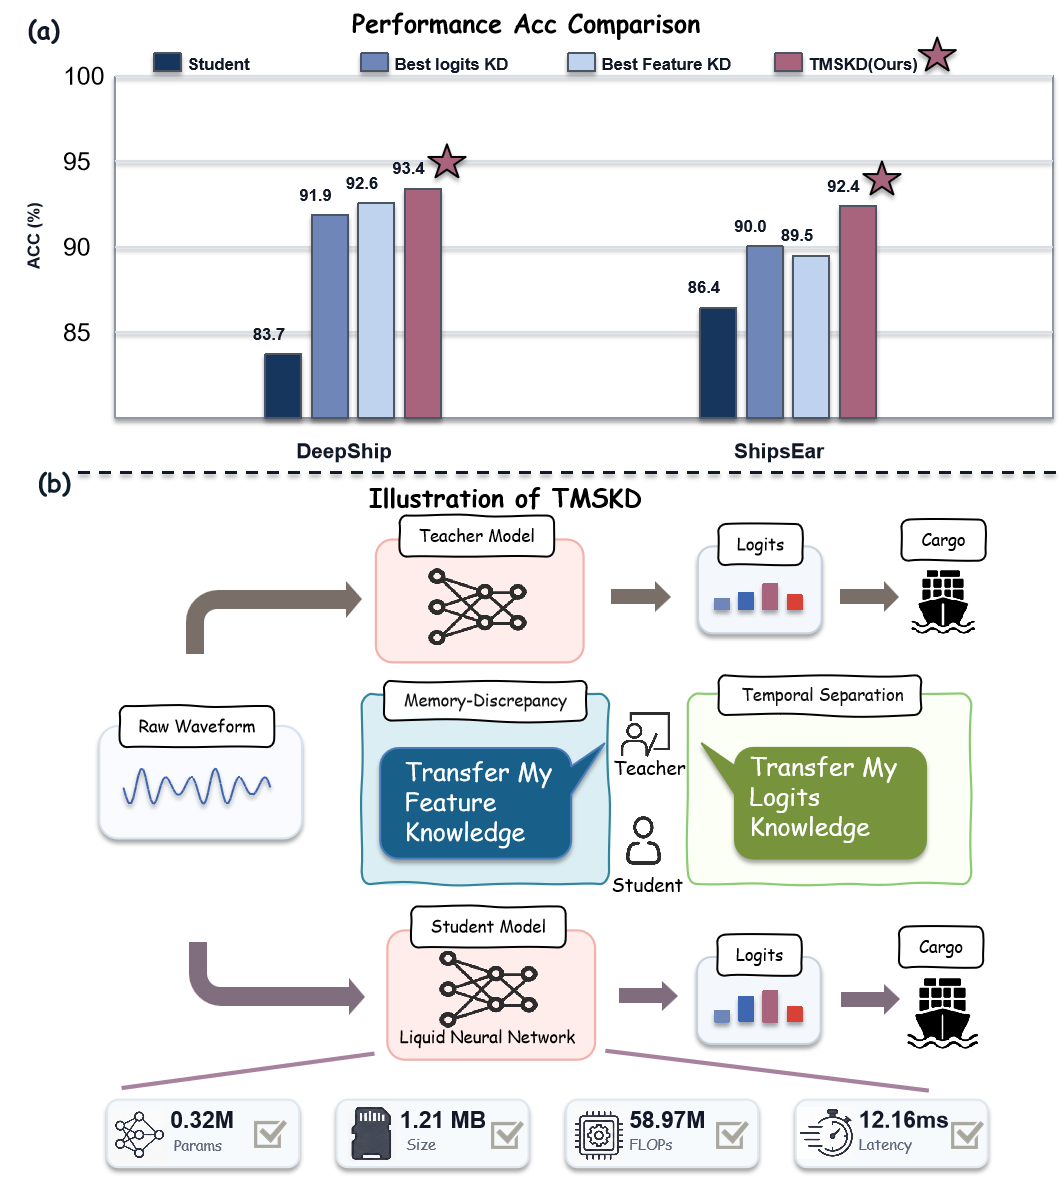
\includegraphics[width=1\linewidth]{figures/Cover_Image.png}
    \caption{(a)TMSKD 在保持极低资源消耗的同时，实现了显著的性能优势。(b) 给定一段水下声学波形，所提出的 TMSKD 框架首先利用 MemKD 对齐异构网络之间的记忆动态轨迹。通过区别于传统的刚性硬对齐，并引入 TS-T 进行基于自适应温度的逐时间步时序对齐，TMSKD 有效地捕捉了长程演变逻辑与细粒度的时序模式。这些提炼出的知识被整合到轻量级 BiTAL 学生网络中，从而产生准确且高效的目标类别预测。}
    \label{fig:placeholder}
\end{figure}
水声目标识别（Underwater Acoustic Target Recognition, UATR）作为海洋监测与防御系统的核心技术，在海洋资源勘探、水下安防以及生态环境监测等领域发挥着不可替代的作用~\cite{Urick1983,Jensen2011}。然而，与陆地声学环境相比，水下声道具有极其复杂的时变、多径效应及环境噪声干扰~\cite{Wenz1962,Medwin2005}，这些复杂的信道特性使得水声信号表现出高度的非平稳性与非线性，极大地增加了从原始信号中提取鲁棒性鉴别特征的难度~\cite{Urick1983,Jensen2011}。更为重要的是，实际的水声识别系统通常部署于水下机器人（AUV）、浮标或传感器节点等边缘设备上，受限于设备的硬件规格，模型的存储空间占用与计算能耗面临严格约束~\cite{Cai2020MobileAUV,Han2016DeepCompression}。因此，如何在有限的计算资源下构建轻量化的识别模型，成为了该领域亟待解决的关键问题。

针对数据稀缺与轻量化部署的双重矛盾，现有的研究主要采取预训练模型微调或模型压缩技术~\cite{Kong2020PANNs,Gou2021KDSurvey}。然而，不同于语音或自然声学信号，水声信号缺乏明确的语义信息（Semantic Information）和音素结构，这导致直接迁移通用音频领域的轻量化预训练模型往往难以捕捉水声信号特有的物理特征，微调效果受限~\cite{Baevski2020Wav2Vec2,Kong2020PANNs,Urick1983,Jensen2011,Medwin2005}。因此，越来越多的研究者将目光转向知识蒸馏（Knowledge Distillation, KD），旨在通过教师网络（Teacher Network）指导轻量化的学生网络（Student Network），以在不增加推理成本的前提下提升模型性能~\cite{Bucila2006Compression,Hinton2015Distilling,Romero2015FitNets}。尽管已有工作在水声领域的蒸馏研究中取得了进展，但我们观察到，目前的轻量化学生网络大多仍依赖于梅尔谱图（Mel-spectrogram）等二维时频特征作为输入。这种做法虽然利用了谱图的视觉纹理特征，但引入了繁琐的预处理计算，违背了端到端（End-to-End）轻量化的初衷。遗憾的是，目前直接使用一维原始波形（Raw Waveform）作为输入的轻量化模型，在特征提取能力上往往显著弱于基于谱图的方法，难以在蒸馏中取得有竞争力的识别精度~\cite{Oord2016WaveNet,Bai2018TCN}。

是否存在一种架构，既能抛弃复杂的谱图转换直接处理原始水声信号，又能具备与谱图输入方法相媲美的特征提取能力？
鉴于此，本文将目光转向液态神经网络。作为一种受生物启发的连续时间递归神经网络，该类网络通过常微分方程（ODEs）对神经元动力学进行建模~\cite{Chen2018NeuralODE,Hasani2021LTC,Hasani2022CfC}，展现出较强的时序因果捕捉能力与鲁棒性。基于这一网络范式，本文设计了双向时序感知液态神经网络（Bidirectional Temporal-Aware Liquid Network, BiTAL），用于处理一维非平稳水声信号。

为了充分挖掘 BiTAL 在水声识别中的潜力，并解决异构网络间知识传递的难题，本文受到时序网络蒸馏思想的启发，提出了一种全新的 MemKD 模块。在传统的蒸馏框架中，由于教师网络与学生网络在参数量级和模型架构上的巨大差异，直接对特征图进行“硬对齐”往往导致学生网络难以收敛或学习到次优特征~\cite{Yim2017FSP,Zagoruyko2017AT,Ahn2019VID}。MemKD 模块则另辟蹊径，它不强求特征数值的逐点逼近，而是旨在将教师网络特征提取器输出的时序演变趋势（Temporal Evolution Trend）以显式的方式传递给学生网络。换言之，我们将教师网络处理音频特征的“思路”与“动态变化规律”传授给学生网络，从而有效规避了因架构差异导致的对齐困难问题。

% 此外，水声信号具有显著的瞬态特性，往往存在特定的“关键频率”或短时特征，这些关键信息在时间轴上的分布是不均匀的，却直接决定了目标的类别判定。传统的基于 Logits 的蒸馏方法通常是对整段音频进行全局池化后的概率分布进行拟合，这种“投票式”的预测方式容易淹没局部关键特征。针对这一问题，我们摒弃了粗粒度的 Logits 蒸馏，转而采用逐时间步（Time-step Wise）的对齐策略。通过强制学生网络在每一个时间步上与教师网络保持一致，模型能够更充分地捕捉并学习不同时刻产生的关键频率特征。
% 这种细粒度的蒸馏范式确保了学生网络不仅学到了“是什么”，更学到了“在哪一时刻”发生了关键变化，从而有效提升了模型对水声目标的判别能力。
% 需要增加自适应温度的描述
此外，水声信号具有明显的瞬态特征，某些关键频率或短时事件可能直接决定目标类别。这些判别性线索在时间轴上分布并不均匀，而传统基于 logits 的蒸馏方法通常只对最终输出分布进行对齐，容易削弱局部时序判别信息。为解决这一问题，我们引入 Temporal Separation with Adaptive Temperature Knowledge Distillation（TS-T），沿时间维度约束教师模型与学生模型之间的语义分布一致性。具体而言，教师 logits 被广播到学生模型的每一个时间步，并与学生的逐时间步 logits 进行对齐，从而引导学生学习关键声学变化发生的时刻。此外，TS-T 对 logits 进行 Z-score 标准化，其中 logits 的标准差作为一种无参数的自适应温度，用于动态调节分布平滑程度~\cite{Sun2024LSKD}。进一步地，TS-T 通过可学习的融合系数平衡逐时间步蒸馏损失与最终 logits 蒸馏损失，使学生模型同时学习细粒度时序线索和稳定的最终决策知识。
% 综上描述创新点To summarize, this article makes the following main contributions.
综上所述，本文主要贡献如下：

\begin{enumerate}[label=\arabic*)]
    \item 我们提出了一种新型知识蒸馏框架，称为时序-记忆结构感知知识蒸馏（Temporal–Memory Structure-Aware Knowledge Distillation, TMSKD），专为水声目标识别（UATR）任务设计。TMSKD融合了基于logits的自适应温度时序分离知识蒸馏（Temporal Separation with Adaptive Temperature Knowledge Distillation, TS-T）与基于特征的记忆差异知识蒸馏（Memory-Discrepancy Knowledge Distillation, MemKD），使学生模型能够同时有效捕捉水声信号中瞬时的类别间关系以及长期的时序记忆模式。
    \item 我们设计了轻量且高效的 BiTAL 学生网络架构，该架构包含五层 CNN 编码器、由 AutoNCP 自动生成神经回路的双向并行交叉切片 CfC（BPCSCfC）模块，以及双分辨率注意力统计池化（Dual-Resolution Attentive Statistics Pooling, DRASP）机制。DRASP 通过全局和局部注意力统计池化，从全局平稳信息和局部瞬态尖峰两个尺度共同建模声学序列，避免依赖单一尺度的注意力统计池化，从而显著提升时频特征的判别性表示能力。
    \item 在两个真实海洋数据集（ShipsEar 5类和DeepShip 4类）上的大量实验表明，所提出的TMSKD显著优于现有的最先进（SOTA）知识蒸馏方法。该框架在保持极低计算复杂度和参数量的同时，实现了准确率的显著提升。特别地，TMSKD为轻量级学生模型带来了可观的性能增益，充分验证了其在资源受限的水下部署场景中的有效性和实用性。
\end{enumerate}


\section{Related Work}

\subsection{水下声学目标识别}

水下声学目标识别（Underwater Acoustic Target Recognition, UATR）旨在通过对水声信号的分析实现对舰船、潜航器等目标的自动分类与识别，是水下监测与海洋安全领域的核心技术之一~\cite{David2016ShipsEar,Irfan2021DeepShip}。由于水下传播环境复杂，信号往往呈现出强非平稳性、长时程依赖性以及显著的背景噪声干扰，使得该任务具有较高挑战性~\cite{Urick1983,Jensen2011,Medwin2005}。

早期方法主要基于人工设计的时域、频域及时频域特征，并结合传统分类器完成识别任务~\cite{David2016ShipsEar,Chen2021LOFAR}。这类方法依赖人工经验，泛化能力有限。

近年来，卷积、循环和 Transformer 等深度网络被广泛应用于水声识别任务，相关方法能够从时频表示或自监督表征中学习判别特征~\cite{Chen2021LOFAR,TFTokenViT,MHTUATR}。然而，这些模型通常采用离散时间建模方式，难以精细刻画连续时间动态变化特性。与此同时，基于预训练语音或通用音频模型的迁移学习方法~\cite{Baevski2020Wav2Vec2,Kong2020PANNs}也被引入水声领域，以利用大规模数据中学习到的通用声学表示能力~\cite{ALSIUATR,CAFJTUATR}。

尽管上述方法在性能上取得了一定提升，但在复杂海洋环境下仍面临模型冗余、对动态变化建模不足以及部署效率受限等问题。因此，构建具有连续时间动态建模能力且参数高效的模型结构成为新的研究方向。

\subsection{液态神经网络}

液态神经网络（Liquid Neural Networks）是一类受小型生物神经系统动力学机制启发的连续时间神经计算模型~\cite{Hasani2021LTC}。其核心思想是通过线性或非线性常微分方程（Ordinary Differential Equations, ODE）描述神经元状态随时间的连续演化过程，从而在理论上更自然地建模时间信号的动态变化~\cite{Chen2018NeuralODE}。

与传统离散层堆叠式网络不同，液态神经网络在每个时间步对隐藏状态进行连续时间更新，使网络具备更强的动态适应能力和可解释性。部分研究提出闭式连续时间（Closed-form Continuous-time）表达形式，使得网络在保证表达能力的同时降低数值求解复杂度~\cite{Hasani2022CfC}。此外，通过构建结构化稀疏连接策略（如自动神经回路生成策略），液态神经网络可以在较低参数规模下实现高效动态建模，具备良好的轻量化潜力~\cite{Lechner2020NCP}。

近年来，液态神经网络在时序预测、机器人控制以及低功耗嵌入式系统中表现出优异性能~\cite{Lechner2020NCP,Hasani2021LTC,Hasani2022CfC}。然而，在水下声学目标识别领域，利用连续时间神经动力学模型刻画水声信号内部复杂动态结构的研究仍相对有限。因此，将液态神经网络引入水声识别任务，有助于增强模型对非平稳信号的动态响应能力，同时兼顾模型轻量化需求。

\subsection{知识蒸馏}

知识蒸馏（Knowledge Distillation, KD）是一种通过教师-学生框架实现模型压缩与性能迁移的有效方法~\cite{Bucila2006Compression,Hinton2015Distilling,Gou2021KDSurvey}。其核心思想是利用性能较强的教师模型所学习到的“软标签”或中间表示，引导参数规模更小的学生模型进行训练，从而在保持较低计算复杂度的同时获得较高识别精度。

经典知识蒸馏方法通常基于输出层的Kullback–Leibler（KL）散度对齐，通过温度系数调节软化分布，以传递类别间的相对关系信息。随后，研究扩展至特征蒸馏、注意力蒸馏和关系蒸馏等方向，通过约束中间层特征或样本间结构关系，进一步提升学生模型的泛化能力~\cite{Romero2015FitNets,Zagoruyko2017AT,Park2019RKD}。

在时序任务中，传统基于最终输出对齐的蒸馏方法难以充分利用时间维度上的动态信息。因此，近年来出现了时序蒸馏策略，通过对每个时间步的预测结果或隐藏状态进行对齐，增强学生模型对时间结构的刻画能力~\cite{Farhadi2019TKD,Wang2023TSKD}。此外，引入温度调节或软标签重加权机制，可以缓解教师与学生分布不一致带来的优化困难~\cite{Sun2024LSKD,Zhou2021WSLD}。

在水声目标识别场景中，由于输入信号具有显著的时序依赖性与动态变化特征，将知识蒸馏与时序建模机制相结合，有助于将大规模预训练模型的判别能力迁移至轻量化动态网络结构中。因此，围绕时序结构感知与动态权重调节的蒸馏策略，成为提升轻量化水声识别模型性能的重要研究方向。

\section{Methodology}
本节首先介绍基于 BiTAL 的水声识别结构，随后详细介绍所提出的\textbf{TMSKD}框架，该框架融合两种\textbf{KD}方法：\textbf{TS-T}和\textbf{MemKD}。
% 修改一下大小
\begin{figure}[htp]
    \centering
    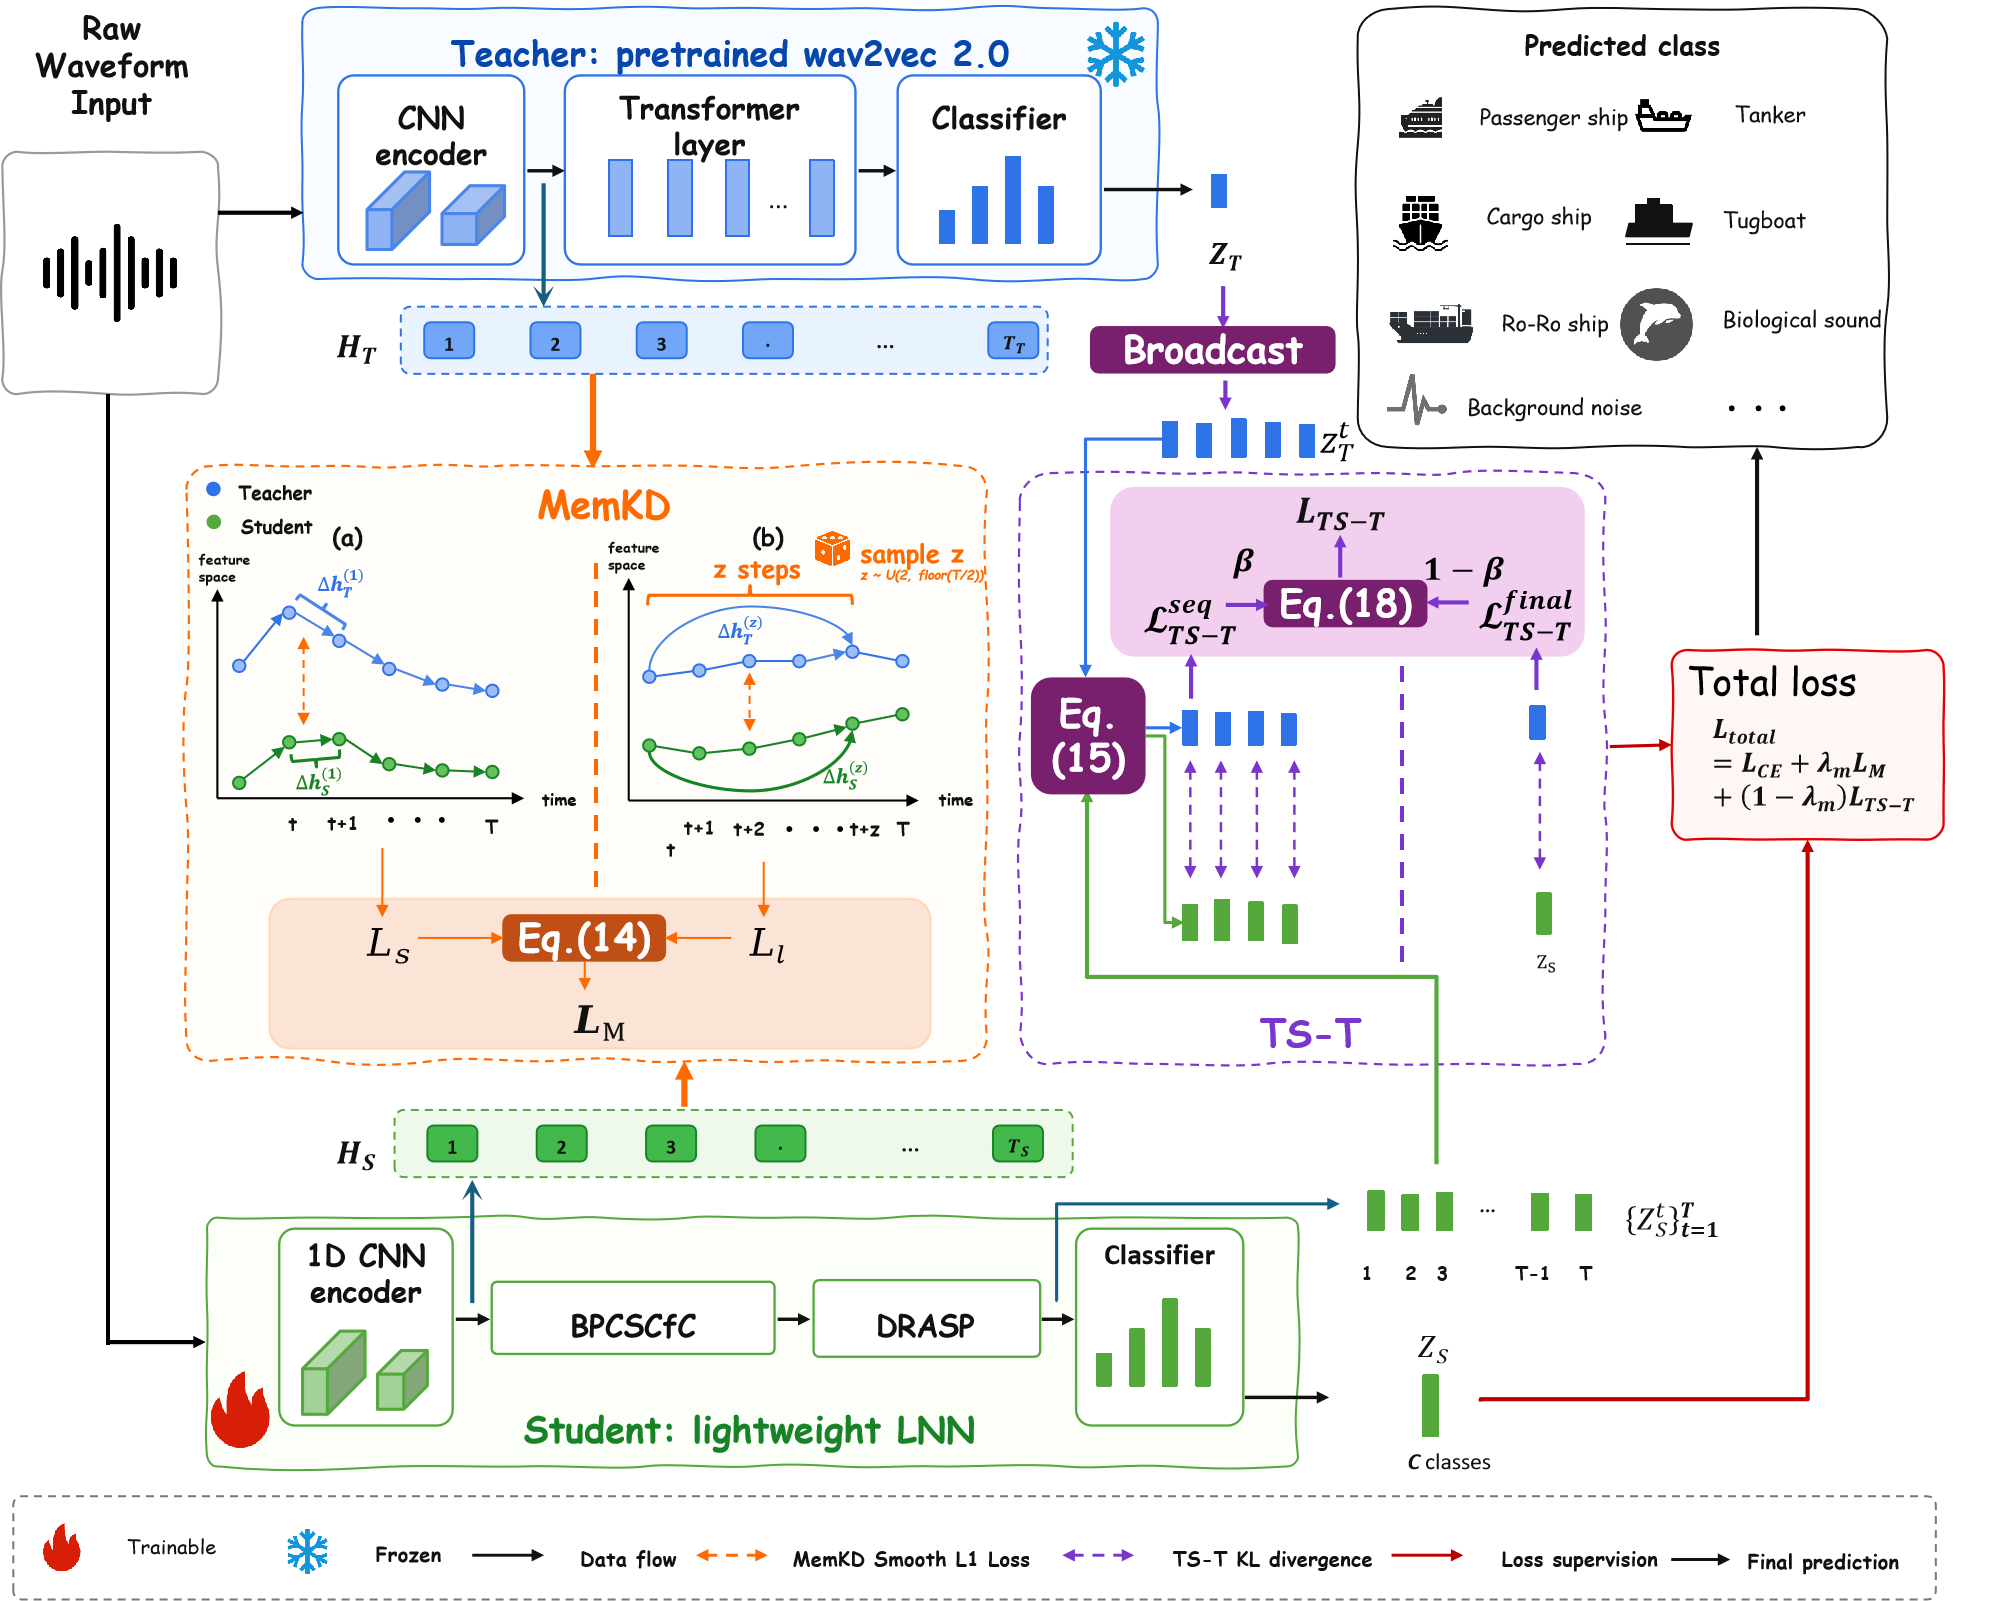
\includegraphics[width=0.7\textwidth]{figures/model_structure_v2.0.png}
    \caption{所提出的水下声学目标识别知识蒸馏框架整体架构。冻结的预训练 wav2vec 2.0 作为教师模型，通过记忆差异知识蒸馏（MemKD）和自适应温度时序分离知识蒸馏（TS-T）指导轻量级 BiTAL 学生网络的训练。学生网络的详细内部结构如图~\ref{fig:student_architecture}所示。}
    \label{fig:structure}
\end{figure}

% \subsection{Preliminaries: Liquid Neural Dynamics}
\subsection{液态神经动力学的初步研究}
针对水声信号具有非平稳性强、时间结构复杂、局部瞬态与长程依赖并存等特点，我们的方法
采用基于闭式连续时间神经网络框架~\cite{Hasani2022CfC}，在$\mathbf{t}$时刻神经动力学方程描述了神经元状态 $\mathbf{x}(t)$的时间演化，由如下线性一阶微分方程定义：
\begin{equation}
\frac{d x(t)}{dt} = -\left[ \tau + f(x(t), I(t), t, \theta) \right] \cdot x(t) + f(x(t), I(t), t, \theta) \cdot A
,
\label{eq:lnn_ode}
\end{equation}
其中，$\tau \in \mathbb{R}^C$用于控制神经元信号变化速率和灵敏度的时间常数，$\theta$代表可学习参数，$I(t)$表示外部输入，$f(x(t), I(t), t, \theta)$是非线性激活函数，$A$是可学习参数向量，使非线性响应的幅度缩放。
该方程刻画了神经元在连续时间上的衰减与外部驱动共同作用下的动态演化过程，从而在时序任务中提升表现力和适应性。

然而，直接对公式~(\ref{eq:lnn_ode})进行数值积分通常计算代价较高。
为此，可以通过对连续时间动力系统进行闭式求解，将其转化为离散时间步上的显式更新形式，从而在保持连续时间建模优势的同时，实现高效稳定的序列建模。
具体而言，在时间步 $t$ 处，公式~(\ref{eq:lnn_ode})的近似解析解由下式给出：
\begin{equation}
\mathbf{x}(t) = \sigma\left(-f(\mathbf{x}, \mathbf{I}; \theta_f) t\right) \odot g(\mathbf{x}, \mathbf{I}; \theta_g) + \left[1 - \sigma\left(-\left[f(\mathbf{x}, \mathbf{I}; \theta_f)\right] t\right)\right] \odot h(\mathbf{x}, \mathbf{I}; \theta_h)
,
\label{eq:cfc_update}
\end{equation}
其中，
$\sigma(\cdot)$ 表示 Sigmoid 门控函数，$\odot$ 表示逐元素乘法，$g(x, I; \theta_g)$根据当前输入$I$ 和前一时刻状态 $x$ 提取当前瞬时的非线性特征。$h(x, I; \theta_h)$ 为补充的特征表示，该算法比基于ODE的网络至少快一个数量级。
相比基于固定离散时间步的 RNN 或 Transformer 结构，该算法使得液态神经元细胞通过显式建模连续时间动力学，能够根据输入信号的动态变化特性灵活调整时间建模尺度，
特别适用于水声信号中存在的多时间尺度动态模式与非平稳特性。
\paragraph{神经回路策略}
在水声目标识别任务中，
输入信号往往包含大量冗余背景信息与非平稳噪声成分，
为提高模型的鲁棒性和参数效率，液态神经元之间不采用全连接结构，
而是通过 Auto Neural Circuit Policy (AutoNCP) 构建结构化稀疏拓扑~\cite{Lechner2020NCP}。
AutoNCP 采用四类神经元的层级架构，包括感觉神经元、中间神经元、命令神经元和运动神经元。其中感觉神经元对应输入特征维度，而中间、命令和运动神经元之间随机连接并构成三层可学习的内部处理层，命令神经元层内部建立循环连接，显著增强了突触对历史隐藏状态的依赖性。

基于公式~(\ref{eq:cfc_update})的液态神经元细胞单元在AutoNCP所定义的连接图上进行状态演化，
使得网络在保持建模能力的同时显著减少参数规模，
并增强对非平稳时序信号的泛化能力。
% \subsection{Student Network: BiTAL Architecture Implementation for Underwater Acoustic Recognition}
\subsection{学生网络：面向水声识别的 BiTAL 架构实现}
为了有效捕捉水下声学信号中的时序动态并兼顾计算效率，基于公式~(\ref{eq:cfc_update})，我们设计了 BiTAL 学生网络，以提升学生模型对复杂海洋环境的适应性，并便于与知识蒸馏框架集成。

对于给定输入的单通道原始水声信号$\mathbf{s} \in \mathbb{R}^{L}$，学生网络首先采用一维卷积编码器将原始时域信号映射为高维时序特征，记为$\mathbf{H}_S\in \mathbb{R}^{B \times T_S \times C}$，其中$B$表示批次大小，$T_S$为时间步，$C$为每个时间步的特征维度~\cite{Oord2016WaveNet,Bai2018TCN}。为同时捕捉$\mathbf{H}_S$中的局部瞬态和长程时序依赖，我们将其输入 BPCSCfC 模块。该模块沿时间维度将序列划分为非重叠窗口，并构建并行信息流以捕捉短程和长程依赖。如图~\ref{fig:student_architecture}所示，所得多尺度时序表示进一步通过 DRASP 的全局与分段局部注意力统计池化进行聚合，并用于最终分类。学生网络的完整前向过程如算法~\ref{alg:student_network}所示。编码器特征$\mathbf{H}_S$用于 MemKD，融合特征$\mathbf{F}_S^t$经线性投影得到供 TS-T 使用的逐时间步 logits $\mathbf{Z}_S^t$。

\begin{figure*}[!t]
    \centering
    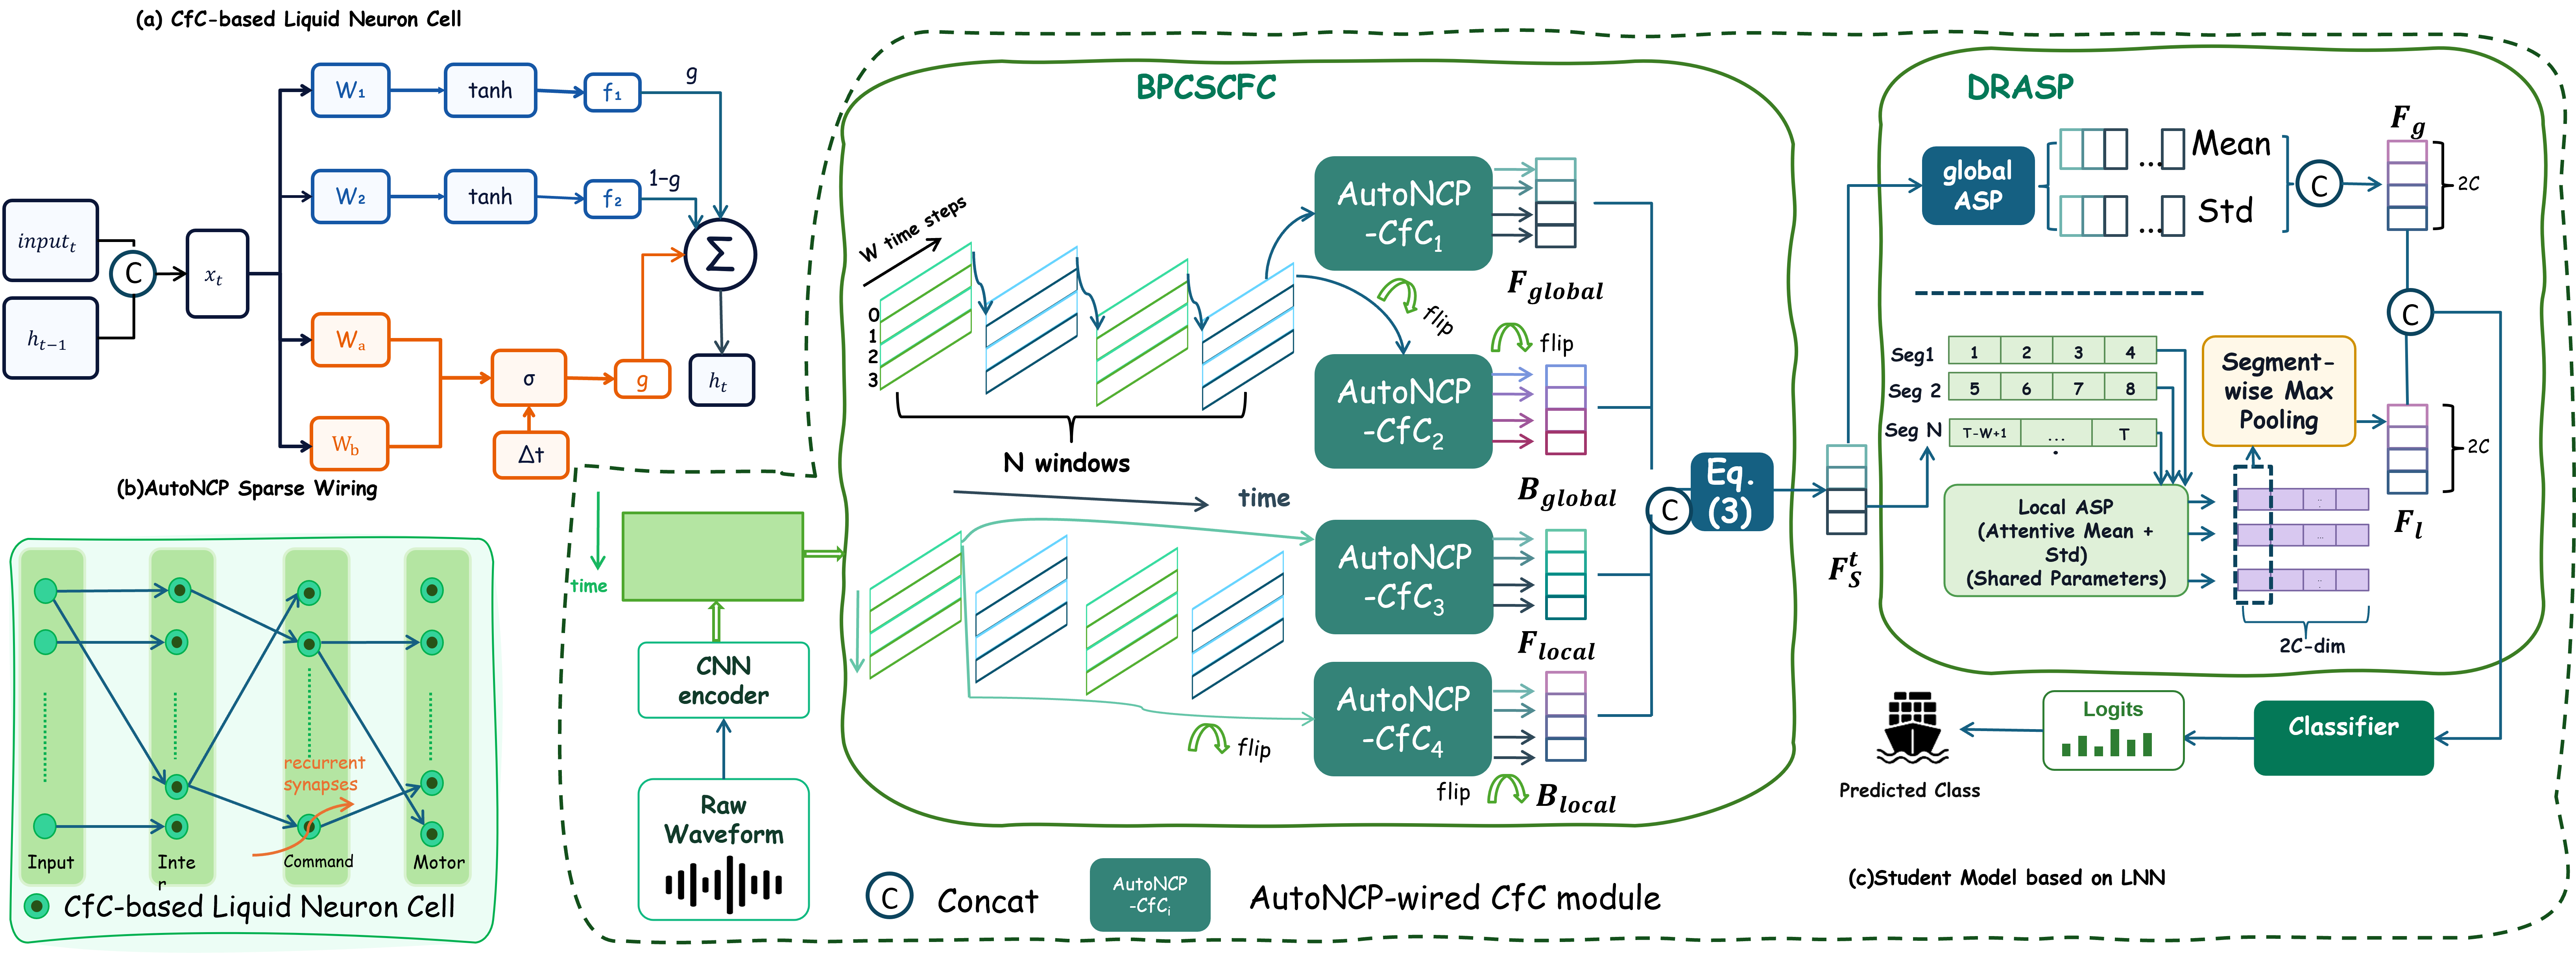
\includegraphics[width=\textwidth]{figures/Detailed Architecture of the Proposed Liquid Neural Student Network.png}
    \caption{所提出的面向水下声学目标识别的 BiTAL 学生网络详细架构。一维 CNN 编码器首先将原始波形转换为时序特征序列，随后由采用 AutoNCP 神经回路连接的 CfC 单元构成的双向并行交叉切片 CfC（BPCSCfC）模块进行建模。双分辨率注意力统计池化（DRASP）模块进一步融合全局注意力统计量与分段局部注意力统计量，形成供分类器使用的语句级表示。}
    \label{fig:student_architecture}
\end{figure*}

\begin{algorithm}[!t]
\caption{面向水声目标识别的 BiTAL 学生网络}
\label{alg:student_network}
\begin{algorithmic}[1]
\Require $\mathbf{s}\in\mathbb{R}^{B\times 1\times L}$；窗口长度 $W$，且 $W\mid T_S$；类别数 $K$
\Ensure $\mathbf{H}_S,\mathbf{F}_S^t\in\mathbb{R}^{B\times T_S\times C}$
\Ensure $\mathbf{Z}_S^t\in\mathbb{R}^{B\times T_S\times K}$；$\mathbf{Z}_S\in\mathbb{R}^{B\times K}$
\State $\mathbf{H}_S \gets \operatorname{Transpose}_{C,T}\big(\operatorname{CNNEncoder}(\mathbf{s})\big)$
\State $N \gets T_S/W$
\State $(\mathbf{H}^{f},\mathbf{H}^{b}) \gets (\mathbf{H}_S,\operatorname{Reverse}_{T}(\mathbf{H}_S))$
\For{$d\in\{f,b\}$} \Comment{正向与反向时序}
    \State $\mathbf{X}^{d} \gets \operatorname{Reshape}(\mathbf{H}^{d},B,N,W,C)$
    \State $\tilde{\mathbf{X}}_{l}^{d} \gets \operatorname{Reshape}(\mathbf{X}^{d},B N,W,C)$
    \State $\tilde{\mathbf{X}}_{g}^{d} \gets \operatorname{Reshape}\big(\operatorname{Permute}_{N,W}(\mathbf{X}^{d}),B W,N,C\big)$
    \State $\mathbf{Y}_{l}^{d} \gets \operatorname{AutoNCP\mbox{-}CfC}_{l}^{d}(\tilde{\mathbf{X}}_{l}^{d})$ \Comment{按公式~(\ref{eq:cfc_update})闭式更新}
    \State $\mathbf{Y}_{g}^{d} \gets \operatorname{AutoNCP\mbox{-}CfC}_{g}^{d}(\tilde{\mathbf{X}}_{g}^{d})$
    \State $\mathbf{O}_{l}^{d} \gets \operatorname{Reshape}(\mathbf{Y}_{l}^{d},B,T_S,C)$
    \State $\mathbf{O}_{g}^{d} \gets \operatorname{Reshape}(\mathbf{Y}_{g}^{d},B,W,N,C)$
    \State $\mathbf{O}_{g}^{d} \gets \operatorname{Reshape}(\operatorname{Permute}_{W,N}(\mathbf{O}_{g}^{d}),B,T_S,C)$
\EndFor
\State $(F_{\mathrm{local}},F_{\mathrm{global}}) \gets (\mathbf{O}_{l}^{f},\mathbf{O}_{g}^{f})$
\State $B_{\mathrm{local}} \gets \operatorname{Reverse}_{T}(\mathbf{O}_{l}^{b})$
\State $B_{\mathrm{global}} \gets \operatorname{Reverse}_{T}(\mathbf{O}_{g}^{b})$
\State $\mathbf{U} \gets \operatorname{Concat}_{C}(F_{\mathrm{local}},F_{\mathrm{global}},B_{\mathrm{local}},B_{\mathrm{global}})$
\State $\mathbf{F}_S^t \gets \operatorname{G}\big(\operatorname{LN}(\mathbf{W}_{p}\mathbf{U}+\mathbf{b}_{p})\big)$
\State $\mathbf{Z}_S^t \gets \operatorname{Linear}_{\mathrm{temp}}(\mathbf{F}_S^t)$ \Comment{蒸馏时用于 TS-T}
\State $\mathbf{F}_g \gets \operatorname{GlobalASP}((\mathbf{F}_S^t)^\top)$
\State $\{\mathbf{F}_{S,m}^t\}_{m=1}^{M} \gets \operatorname{PadAndSegment}_{W}(\mathbf{F}_S^t)$
\For{$m=1$ to $M$}
    \State $\mathbf{F}_{l,m} \gets \operatorname{LocalASP}((\mathbf{F}_{S,m}^t)^\top)$ \Comment{共享局部 ASP 参数}
\EndFor
\State $\mathbf{F}_l \gets \operatorname{MaxPool}_{m}(\{\mathbf{F}_{l,m}\}_{m=1}^{M})$
\State $\mathbf{F}_{\mathrm{pooled}} \gets \operatorname{Concat}_{C}(\mathbf{F}_g,\mathbf{F}_l)$
\State $\mathbf{Z}_S \gets \operatorname{Classifier}(\mathbf{F}_{\mathrm{pooled}})$
\State \Return $\mathbf{Z}_S$, $\mathbf{Z}_S^t$, $\mathbf{F}_S^t$, $\mathbf{H}_S$ \Comment{$\mathbf{H}_S$ 用于 MemKD}
\end{algorithmic}
\end{algorithm}

具体而言，对重排后的序列特征输入按照公式~(\ref{eq:cfc_update})进行状态演化：将$\mathbf{H}_S$重排为$\mathbf{X}_l\in \mathbb{R}^{B \times N \times W \times C}$，其中$N=T_S/W$为窗口数量，$W$为每个窗口的时间步长度，将批次维度与窗口数量维度进行合并得到$\tilde{\mathbf{X}}_l \in \mathbb{R}^{(B \cdot N) \times W \times C}$。前向局部流捕捉窗口内部相邻时间步的短程依赖，沿原始时间轴独立处理每个长度为 $W$ 的窗口得到前向局部时序特征$F_{local}$；为引入短程模式的反向上下文信息，反向局部流将输入序列沿时间维度翻转后执行与前向局部流相同的处理，再恢复为原始时间顺序，得到反向局部时序特征$B_{local}$。为了建模跨窗口的长程依赖关系，将$\mathbf{H}_S$重排为$\mathbf{X}_g\in \mathbb{R}^{B \times W \times N \times C}$,将批次维度与窗口维度进行合并，得到$\tilde{\mathbf{X}}_g \in \mathbb{R}^{(B \cdot W) \times N \times C}$，该重排操作将原始时间序列按窗口位置重新组织，使同一窗口位置的时间步形成新的跨窗口序列。
前向全局流沿跨窗口序列对长度为$N$ 的特征序列进行建模，得到前向全局时序特征$F_{global}$；对时间翻转后的输入执行相同全局处理并恢复原始时间顺序，得到反向全局时序特征$B_{global}$。四路特征在通道维度上进行拼接，经过线性投影、层归一化和激活函数，得到细粒度时序序列$\mathbf{F_S^t}\in \mathbb{R}^{B \times T_S \times C}$状态：
\begin{equation}
\mathbf{F_S^t}
=
\operatorname{G}
\Big(
\operatorname{LN}
\big(
\mathbf{W}\cdot Concat(F_{local},F_{global},B_{local},B_{global})
+ \mathbf{b}
\big)
\Big),
\quad
\mathbf{F_S^t} \in \mathbb{R}^{B \times T_S \times C},
\end{equation}其中$\operatorname{G}(\cdot)$表示激活函数，$\operatorname{LN}$表示层归一化，$Concat(\cdot)$为连接算子，$\mathbf{W}$ 与 $\mathbf{b}$ 为可学习参数。

水声信号同时包含全局声学特性(如音色、频谱能量分布)和局部瞬态事件(如机械启动、突发噪声)，单一尺度的池化难以同时捕获这两类特征，我们设计了双分辨率注意力统计池化模块，构建全局和局部两条并行分支。
具体而言，全局分支直接对输入序列$\mathbf{F_S^t}$（转置为 $\textbf{F}\in \mathbb{R}^{B \times C \times T_S}  $）计算注意力统计池化：
首先计算注意力权重 $  \alpha \in \mathbb{R}^{B \times T_S}  $：
\begin{equation}
\alpha = \operatorname{Softmax}_T \left( \mathbf{W}_{\alpha} \cdot \tanh(\mathbf{W}_{\beta} \cdot \mathbf{F}) \right),
\end{equation}
其中 $  \mathbf{W}_{\alpha} \in \mathbb{R}^{1 \times C'}  $ 和 $  \mathbf{W}_{\beta} \in \mathbb{R}^{C' \times C}  $ 为可学习的投影矩阵。随后，计算加权均值 $  \mu  $ 和标准差 $  \sigma  $，
\begin{equation}
\mu = \sum_{t=1}^{T_S} \alpha_t \cdot \mathbf{F}_t, \quad
\sigma = \sqrt{ \sum_{t=1}^{T_S} \alpha_t \cdot (\mathbf{F}_ t - \mu)^2 + \epsilon },
\end{equation}
其中 $  \epsilon=10^{-6}  $ 为数值稳定性常数，最终拼接均值与标准差为全局统计特征：
\begin{equation}
\mathbf{F}_{g}=Concat(\mu_g,\sigma_g) \in \mathbb{R}^{B \times 2C}
\end{equation}
局部分支首先将输入序列划分为多个短时片段,然后对每个片段分别应用注意力统计池化,在片段维度上通过最大池化提取最显著的局部特征$F_l \in \mathbb{R}^{B \times 2C}$。
并将全局和局部分支的统计量沿通道维度拼接后得到池化特征 $  \mathbf{F}_{\text{pooled}} \in \mathbb{R}^{B \times 4C}  $。
局部模块突出瞬态信息，全局模块提取整体平稳信息，该模块有效减少了冗余信息，提升了对水声信号多尺度特征的敏感性。
最终，池化特征 $\mathbf{F}_{\text{pooled}}$ 输入分类器进行水声分类识别。
该学生网络整体轻量高效，适用于水下实际部署，同时适用于通过后续知识蒸馏机制从教师模型继承高级语义知识。
% 该架构与TMSKD蒸馏方法无缝集成，通过MemKD和TS-T损失指导学生学习教师的时序记忆和分布知识，实现准确率提升10\%以上。
% \subsection{Memory-Discrepancy Knowledge Distillation}
\subsection{基于记忆差异的知识蒸馏}
\label{subsec:memkd}

学生模型中间层输出的序列特征本质上是隐藏状态在时间轴上的连续演进，它将声学输入编码为高维空间的动态轨迹。然而，对于具有强时序相关性的水声信号，传统的对齐学生和教师模型特征图的方法很难学习到有效的分类模式，且易受异构网络间特征分布不一致的影响。
为此，本文将聚焦于“动态轨迹拟合”，利用隐藏状态序列的潜在演变模式。具体来说，短期记忆差异捕获了声学信号在极短时间内的瞬时物理变化，而长期记忆差异则有效缓解网络的遗忘问题。因此，我们提出MemKD模块，旨在学生模型可以学习到“教师模型是如何一步步推导出这个结果的”，使LNN能够跨越架构差异深度学习教师网络处理复杂声学时序的“逻辑经验”。

MemKD的输入是学生和教师模型的中间特征映射。$\mathbf{H}_S$为学生模型编码器深层的时序隐藏状态，教师模型
% （wav2vec 2.0）
对应层的特征为 $  \mathbf{H}_T \in \mathbb{R}^{B \times T_t \times D_t}  $，其中通常 $  T_t > T_S  $ 且 $D_t \gg C$。

首先，考虑到水声信号的时序连续性和多尺度传播特性，因此我们采用平滑的一维线性插值进行时间对齐。将教师序列在时间维度上重采样到学生的时间长度：
\begin{equation}
\hat{\mathbf{H}}_T = \text{Interp}(\mathbf{H}_{T}, T_S).
\end{equation}
其中 $\text{Interp}(\cdot)$ 表示沿时间维度进行的线性插值操作。为表述简洁，以下仍记$\hat{\mathbf{H}}_T$为$\mathbf{H}_T$。

MemKD 的核心思想在于刻画不同时间跨度下的\textbf{记忆差异}。给定时间偏移 $z$，我们分别计算教师与学生的状态变化量：
\begin{equation}
\Delta \mathbf{H}^t_{(\cdot)}
= \mathbf{H}^{t+z}_{(\cdot)} - \mathbf{H}^{t}_{(\cdot)},
\end{equation}
其中 $(\cdot)$ 表示教师或学生。

为消除特征维度差异带来的影响，上述差分向量进一步通过当前状态范数进行归一化：
\begin{equation}
\mathbf{F}^{(\cdot)}_t
= \frac{\Delta \mathbf{H}^t_{(\cdot)}}
{\|\mathbf{H}^t_{(\cdot)}\|_2 + \epsilon}.
\end{equation}

由于异构网络之间方向信息不可直接对齐，我们仅保留归一化向量的幅度信息：
\begin{equation}
\mathbf{M}^{(\cdot)}_t
= \left\|
\mathbf{F}^{(\cdot)}_t
\right\|_2.
\end{equation}

随后采用 Smooth L1 Loss 对教师与学生的记忆轨迹进行匹配：
\begin{equation}
\mathcal{L}_{\text{MemKD}}(z)
=
\frac{1}{T-z}
\sum_{t=1}^{T-z}
\mathrm{SmoothL1}
\Big(
\mathbf{M}^{S}_t,
\mathbf{M}^{T}_t
\Big).
\end{equation}

考虑到水声信号同时包含局部瞬态事件与全局传播模式，我们设计短程与长程两个互补分支。

\paragraph{(1) 短程记忆差异}
% \paragraph{(1)Short-term Memory Discrepancy}

当 $z=1$ 时，短程记忆损失为：
% \begin{equation}
% \mathcal{L}_{\text{short}}
% =
% \frac{1}{T-1}
% \sum_{t=1}^{T-1}
% \mathrm{SmoothL1}
% \Big(
% \mathbf{M}^{S}_t(z{=}1),
% \mathbf{M}^{T}_t(z{=}1)
% \Big),
% \end{equation}
\begin{equation}
    \mathcal{L}_{\text{s}}=\mathcal{L}_{\text{MemKD}}(z=1),
\end{equation}
用于捕捉相邻帧之间的局部动态变化。

\paragraph{(2) 长程记忆差异}
% \paragraph{(2)Long-term Memory Discrepancy}
在每个训练步随机采样
\(
z \sim \mathcal{U}\big(2,\lfloor T/2 \rfloor\big)
\)，
长程记忆损失定义为：
% \begin{equation}
% \mathcal{L}_{\text{long}}
% =
% \frac{1}{T-z}
% \sum_{t=1}^{T-z}
% \mathrm{SmoothL1}
% \Big(
% \mathbf{M}^{S}_t(z),
% \mathbf{M}^{T}_t(z)
% \Big),
% \end{equation}
\begin{equation}
    \mathcal{L}_{\text{l}}=\mathcal{L}_{\text{MemKD}}(z),
\end{equation}
用于建模跨较长时间跨度的平稳依赖关系。

最终 MemKD 目标损失为：
% \begin{equation}
% \mathcal{L}_{\text{MemKD}}
% =
% 0.5\, \mathcal{L}_{\text{short}}
% +
% 1.0\, \mathcal{L}_{\text{long}}.
% \end{equation}
\begin{equation}
\mathcal{L}_{\text{M}}
=
\lambda_s\, \mathcal{L}_{\text{s}}
+
\lambda_l\, \mathcal{L}_{\text{l}}.
\end{equation}
% 改一下a,b参数
% wav2vec 2.0 ->教师网络
% 该策略能够有效引导学生模型学习 wav2vec 2.0 中蕴含的长期时序依赖关系，而无需显式对齐高维特征空间。
其中 $\lambda_s$ 和 $\lambda_l$ 为固定超参数，用于平衡短期瞬态特征与长期时序模式的学习权重。该策略能够有效引导学生模型学习教师模型中蕴含的长期时序依赖关系，而无需显式对齐高维特征空间。


\subsection{自适应温度的时序分离知识蒸馏}
% \subsection{Temporal Separation with Adaptive Temperature Knowledge Distillation}
\label{subsec:tser}

与传统仅在最终输出层进行分布对齐的知识蒸馏方法不同，
TS-T在时间维度上对教师与学生的语义演化轨迹进行约束，
从而显式引导学生模型学习教师在不同时刻的判别动态。

教师模型输出的Logits表示记为
$\mathbf{Z}_{T} \in \mathbb{R}^{B\times K}$，
学生模型将$\mathbf{F_S^t}$经过线性变化转换为
$\mathbf{Z}^{t}_S \in \mathbb{R}^{B \times T_s \times K}$，学生模型的分类中的logits为$\mathbf{Z}_S \in \mathbb{R}^{B \times K}$，
其中 $K$是水下声音识别种类(e.g.,$K=5$ for ShipsEar and $K=4$ for DeepShip)。


将温度系数 $\tau$ 显式地定义为Logit的样本标准差，对教师模型和学生模型的Logit进行Z-score标准化处理，从而实现了无参数的自适应温度调节。对于任意 Logit 向量 $\mathbf{z}$，其标准化过程定义如下：\begin{equation}
\hat{z}_i = \frac{z_i - \mu_\mathbf{z}}{\sigma_\mathbf{z} + \epsilon}.
\end{equation}其中 $\mu_\mathbf{z}$ 和 $\sigma_\mathbf{z}$ 分别表示 $\mathbf{z}$ 在类别维度上的均值和标准差，$\epsilon$ 为防止除零的极小常数。在此框架下，标准差 $\sigma_\mathbf{z}$ 实际上充当了自适应温度系数的角色，动态地调整了概率分布的平滑度。


为了使学生网络在每个时间步的学习都受到教师网络输出分布的指导，
我们将$\mathbf{Z}_{T}$ 沿时间维度复制并广播，
得到 $\mathbf{Z}_{T}^{t} \in \mathbb{R}^{B \times T_s \times K}$，
从而与学生模型的$\mathbf{Z}_S^{t}$ 进行对齐。
第 $i$ 个样本在时间步 $t$ 的教师与学生 logits 向量标准化后的形式记为
$\hat{\mathbf{z}}_T^{(i,t)}$ 和 $\hat{\mathbf{z}}_S^{(i,t)}$，
时序蒸馏损失 $\mathcal{L}_{TS-T}^{seq}$ 通过对每一帧的
KL 散度进行加权求和得到：

\begin{equation}
\mathcal{L}_{TS-T}^{seq}
=
\frac{1}{B}
\sum_{i=1}^{B}
\sum_{t=1}^{T_s}
w_t
D_{KL}
\left(
\sigma(\hat{\mathbf{z}}_{T}^{(i,t)})
\|
\sigma(\hat{\mathbf{z}}_{S}^{(i,t)})
\right).
\end{equation}

其中 $\sigma(\cdot)$ 表示 Softmax 函数，
$w_t$ 为时间权重系数（本工作采用均匀权重），
$D_{KL}(\cdot)$ 表示 Kullback–Leibler (KL) 散度，
用于度量教师模型与学生模型在每个时间步预测分布之间的差异。

\begin{equation}
    \mathcal{L}_{\text{TS-T}}^{\text{final}}= D_{KL}(Z_S || Z_T),
\end{equation}
为保持整体类别分布一致性，
同时引入最终输出层蒸馏损失
$\mathcal{L}_{\text{TS-T}}^{\text{final}}$保证模型最终分类决策的准确性。
TS-T蒸馏目标损失为：

\begin{equation}
\mathcal{L}_{\text{TS-T}}
=
\beta \cdot \mathcal{L}_{\text{TS-T}}^{\text{seq}}
+
(1 - \beta)\cdot
\mathcal{L}_{\text{TS-T}}^{\text{final}},
\end{equation}
其中 $\beta$ 为可学习融合系数。TS-T主要约束时间维度分布一致性，而 MemKD 进一步对隐藏结构进行学习，两者互补。
\subsection{总损失函数}
% \subsection{Overall Training Loss}
\label{subsec:total_loss}

整体框架如图~\ref{fig:structure}采用教师–学生范式，
% 其中教师模型选用预训练的 wav2vec~2.0，并在训练过程中保持参数冻结；
对于学生模型，我们采用基于闭式连续时间液态结构的 BiTAL，用于完成最终的下游任务预测。
总结来说，整体训练目标定义为：
\begin{equation}
\mathcal{L}_{\text{total}} = \mathcal{L}_{\text{CE}} + \lambda_m \, \mathcal{L}_{\text{M}} + (1 - \lambda_m) \, \mathcal{L}_{\text{TS-T}}
\end{equation}
其中，$\mathcal{L}_{\text{CE}}$代表学生模型的分类损失，即标准交叉熵损失。$\lambda_m$是自适应加权的平衡蒸馏损失的权重。

\section{EXPERIMENTS}
\subsection{Experimental Setup}
\subsubsection{基准数据集}
% \subsubsection{Benchmark Data Sets}
本文实验采用两个真实海洋数据集进行验证：ShipsEar\cite{David2016ShipsEar}和 DeepShip\cite{Irfan2021DeepShip}。ShipsEar 数据集包含5类水下声学目标，包括客船、拖船、货船、背景噪声和海洋生物，总计约90段录音，总时长超过4小时。这些录音采集自西班牙沿海地区，使用采样率为52.7 kHz的设备。DeepShip 数据集包含4类船舶辐射噪声，包括客船、油轮、货船和滚装船，总计265段录音，总时长超过47小时。这些录音来源于全球不同海域，使用采样率为32 kHz的设备。
为确保公平比较，所有音频信号统一重采样为16 kHz，并截取为固定长度（3秒）。数据集按8:1:1的比例划分为训练集、验证集和测试集。Details of the two
datasets are provided in Table ~\ref{tab:dataset}.
\begin{table}[htbp]
\centering
\caption{Configurations of DeepShip and ShipsEar Datasets}
\begin{tabular}{l|cc}
\hline
Configurations & DeepShip & ShipsEar \\
\hline
Dataset size & 53155 & 3738 \\
Category     & 4     & 5    \\
Location     & Canada Strait of Georgia & Spanish Atlantic Coast \\
Equipment    & icListen AF Hydrophone   & digitalHyd SR-1 \\
\hline
\end{tabular}
\label{tab:dataset}
\end{table}
\subsubsection{实验设置}
我们利用 PyTorch 框架构建整个模型架构并基于NVIDIA RTX 4090 GPU开展实验，
% 实验基于PyTorch框架实现，运行于NVIDIA RTX 4090 GPU
% （24 GB显存）
其中教师模型选用预训练的Wav2Vec 2.0音频分类网络，并在蒸馏过程中冻结其参数。
% （约164M参数），其在ShipsEar和DeepShip上的预训练准确率分别为85.2\%和92.4\% 。
% 学生模型采用自定义连续时间网络(Liquid Continuous Network Student,LCN)架构，参数量约150K，FLOPs约120M。
% 学生模型的参数量约150K，FLOPs约120M。
蒸馏过程使用AdamW优化器，初始学习率为5e-4，
% 批大小为32，
总训练轮次为200，训练中批次大小是根据各数据集的特征和内存需求选定的，以确保模型能够稳定收敛。
% The batch size was selected according to the characteristics and memory requirements of each dataset to ensure stable convergence.
TMSKD方法中，MemKD组件的内存差异计算引入短程（z=1）和远程（z=动态随机，范围2-8）损失,MemKD损失中的短期与长期权重参数分别固定为 $\lambda_s= 0.5  $ 和 $\lambda_l= 1.0  $;TS-T组件的时序分离采用自适应温度
% 可学习温度（初始值为4.0）
，可学习权重$\beta$自适应调整 $\mathcal{L}_{\mathrm{TS\mbox{-}T}}^{\mathrm{seq}}$和$\mathcal{L}_{\mathrm{TS\mbox{-}T}}^{\mathrm{final}}$。
% 这两个参数在整个训练过程中不参与梯度计算，始终保持恒定值。
蒸馏损失函数结合标签损失和软损失，本实验采用 10折交叉验证来评估模型的性能。我们将数据集随机划分为 10 个互不相交的子集，在每一轮实验中，轮流选取其中一个子集作为验证集，其余 9 个子集作为训练集，最终报告 10 次实验结果的 均值。
% $\alpha$参数初始化为0.0并在训练中学习。数据增强包括随机噪声注入和时频掩码，以提升模型对海洋环境变异的鲁棒性。
% 所有实验重复5次取平均值，以减少随机性影响。
\subsubsection{评估指标}
我们通过准确率(ACC)、F1-score, and area under curve (AUC)来评估算法效果。准确率（ACC）衡量正确分类实例占总实例的比例，用于量化识别性能。
% ACC表述为：
% \begin{equation}
%     ACC = \frac{\sum_{i=1}^{M} \sum_{j=1} s_{ij}}{\sum_{i=1}^{M} \sum_{j=1}^{M} s_{ij}}
% \end{equation}
% where $M$ is the number of categories. $s_{ij}$ denotes the count of instances classified as $i$ that are predicted to belong to $j$. F1-score provides a balance between precision and recall, especially when the data set is imbalanced. F1-score can be written as
辅助指标包括F1分数（F1-Score），以处理类别不平衡，以及曲线下面积(AUC)，用于评估模型在不同阈值下的分类能力。此外，为全面评估模型的部署效率，统计各模型的参数量（Parameters）、模型大小（Model Size）、浮点运算次数（FLOPs）以及推理延迟（Latency）~\cite{Han2016DeepCompression}。其中，参数量和模型大小用于衡量存储开销，FLOPs用于反映理论计算复杂度，而Latency在单GPU环境下以毫秒（ms）为单位进行测试用于衡量实际推理效率。我们从模型复杂度与实际运行效率两个方面进行分析。
% 此外，评估模型压缩效果，通过参数量（Params）和浮点运算量（FLOPs）衡量轻量级程度；推理时间（Inference Time）在单GPU上测试，以毫秒为单位，模拟实际部署效率。
% 蒸馏效率通过学生模型相对于教师的相对提升率（Improvement Ratio）计算，即（学生ACC - 基线学生ACC）/ 教师ACC \times 100\%。
这些指标确保全面评估TMSKD在精度、效率和鲁棒性上的优势。
\subsection{对比实验}
\subsubsection{Comparison With the SOTA KD Methods}

我们提出的TMSKD 方法与21种经典或流行的state-of-the-art(SOTA)知识蒸馏方法进行了对比，包括基于 logits 的方法（如 KD~\cite{Hinton2015Distilling}、DKD~\cite{Zhao2022DKD}、NKD~\cite{Yang2023NKD}、LSKD~\cite{Sun2024LSKD}、SDD~\cite{Wei2024SDD} 和 WSLD~\cite{Zhou2021WSLD}）以及基于特征的蒸馏方法（如 AT~\cite{Zagoruyko2017AT}、SP~\cite{Tung2019SP}、FSP~\cite{Yim2017FSP}、RKD~\cite{Park2019RKD}、PKT~\cite{Passalis2018PKT}、MGD~\cite{Yang2022MGD} 和 MKD~\cite{Lao2023MKD} 等）。
从表 \ref{tab:distillation_results} 可以看出，所提出的 TMSKD 方法在两个数据集上的所有评价指标（ACC、F1-score 和 AUC）均取得了最优性能。具体来说，在 DeepShip 数据集上，TMSKD 在 ACC、F1-score 和 AUC 上分别达到 93.41\%、93.40\% 和 99.17\%，相较于次优方法分别提升了 0.85\%、0.87\% 和 0.10\%。在 ShipsEar 数据集上，TMSKD 同样表现出显著优势，在 ACC、F1-score 和 AUC 上分别达到 92.39\%、92.34\% 和 98.84\%，相比第二名方法提升了 2.36\%、2.96\% 和 0.53\%。
进一步地，与未蒸馏的学生模型相比，TMSKD 在 DeepShip 数据集上分别提升了 5.67\%、5.68\% 和 1.47\%，在 ShipsEar 数据集上提升了 4.14\%、4.35\% 和 1.01\%，说明所提出方法能够有效弥补学生模型性能不足的问题。
从不同蒸馏范式来看，基于 logits 的方法整体性能较为稳定，但受限于仅利用输出分布信息，其性能提升有限；而基于特征的方法（如 FSP 和 MKD）在部分指标上取得了较优结果，说明中间特征对齐在一定程度上有助于知识迁移。然而，这些方法通常忽略了时序建模和动态记忆特性。
相比之下，TMSKD 同时结合了时序信息建模与记忆结构约束，通过对学生网络动态状态演化过程的显式对齐，实现了更充分的知识迁移，从而在所有指标上均取得显著优势。这也验证了在水声目标识别任务中，引入时序-记忆结构感知蒸馏机制的有效性和必要性。
\begin{table*}[!htbp]
\centering
\caption{Performance Comparison of Different Distillation Methods on DeepShip and ShipsEar Data Sets. Top three results are colored in \textcolor{red}{red}, \textcolor{blue}{blue}, and \textcolor{green}{green}, respectively.
$\uparrow$ indicates the improvement of TMSKD over the second-best method.
$\uparrow\uparrow$ denotes the improvement of TMSKD over the student model.}
\label{tab:distillation_results}
\small
\setlength{\tabcolsep}{4pt}

\begin{tabular}{c|c|c|c|c|c|c|c}
\toprule

\multirow{2}{*}{Distillation Mechanism} &
\multirow{2}{*}{Method} &
\multicolumn{3}{c|}{DeepShip} &
\multicolumn{3}{c}{ShipsEar} \\

& & ACC & F1-score & AUC & ACC & F1-score & AUC \\

\midrule

\multirow{2}{*}{\makecell{Baseline \\ (No KD)}}
& Teacher (Wav2vec 2.0) & 98.56 & 98.56 & 99.93 & 94.66 & 94.66 & 99.63 \\
& Student (BiTAL) & 83.74 & 87.72 & 97.70 & 86.44 & 87.99 & 97.83 \\

\midrule

\multirow{6}{*}{Logits}
& KD\cite{Hinton2015Distilling}  & 91.86 & 91.83 & 99.03 & \textcolor{blue}{90.03} & \textcolor{blue}{89.38} & 98.27 \\
& DKD~\cite{Zhao2022DKD} & \textcolor{green}{92.12} & \textcolor{green}{92.08} & 98.94 & 88.70 & 87.78 & 97.78 \\
& NKD~\cite{Yang2023NKD} & 91.75 & 91.72 & 98.91 & 89.10 & 87.73 & 98.09 \\
& LSKD~\cite{Sun2024LSKD} & 91.35 & 91.32 & 98.89 & 89.10 & 88.71 & 98.21 \\
& SDD~\cite{Wei2024SDD} & 91.23 & 91.19 & 98.79 & 89.10 & 88.38 & \textcolor{green}{98.28} \\
& WSLD~\cite{Zhou2021WSLD} & 91.37 & 91.32 & 98.89 & 88.43 & 87.89 & 98.12 \\

\midrule

\multirow{15}{*}{Feature}
& AT~\cite{Zagoruyko2017AT} & 90.80 & 90.77 & 98.76 & 89.49 & \textcolor{green}{88.98} & 98.02 \\
& SP~\cite{Tung2019SP} & 91.26 & 91.22 & 98.88 & 88.30 & 87.88 & 98.06 \\
& FSP~\cite{Yim2017FSP} & \textcolor{blue}{92.56} & \textcolor{blue}{92.53} & \textcolor{blue}{99.07} & 88.43 & 86.86 & 97.62 \\
& NST~\cite{Huang2017NST} & 90.72 & 90.69 & 98.89 & 87.50 & 86.87 & 97.71 \\
& RKD~\cite{Park2019RKD} & 91.32 & 91.28 & 98.95 & 87.77 & 86.55 & 97.38 \\
& PKT~\cite{Passalis2018PKT} & 89.47 & 89.42 & 98.62 & 88.56 & 87.33 & 97.92 \\


& FreeKD~\cite{Zhang2024FreeKD} & 91.68 & 91.63 & 98.90 & 87.23 & 86.33 & 97.81 \\
& CC~\cite{Peng2019CC} & 91.20 & 91.16 & 98.87 & 88.96 & 88.22 & 98.08 \\
& VID~\cite{Ahn2019VID} & 91.20 & 91.15 & 98.84 & 88.30 & 87.75 & 98.08 \\
& VKD~\cite{Miles2024VKD} & 89.47 & 89.40 & 98.51 & 87.77 & 86.93 & 97.67 \\
& MGD~\cite{Yang2022MGD} & 91.12 & 91.09 & 98.90 & 88.43 & 87.73 & 97.94 \\
& DiffKD~\cite{Huang2023DiffKD} & 89.04 & 88.98 & 98.44 & 88.56 & 87.95 & 98.07 \\
& MKD~\cite{Lao2023MKD} & 92.02 & 91.99 & \textcolor{green}{99.04} & \textcolor{green}{89.36} & 88.71 & \textcolor{blue}{98.31} \\
& CAT-KD~\cite{Guo2023CATKD} & 89.40 & 89.33 & 98.49 & 87.63 & 86.65 & 97.92 \\
& ICKD~\cite{Liu2021ICKD} & 91.24 & 91.18 & 98.96 & 84.71 & 83.81 & 97.22 \\
\midrule

\rowcolor{gray!15}
& \textbf{TMSKD (Ours)} &
\textcolor{red}{93.41} &
\textcolor{red}{93.40} &
\textcolor{red}{99.17} &
\textcolor{red}{92.39} &
\textcolor{red}{92.34} &
\textcolor{red}{98.84} \\

& $\uparrow$ & \textbf{+0.85} & \textbf{+0.87} & \textbf{+0.10} & \textbf{+2.36} & \textbf{+2.96} & \textbf{+0.53} \\

& $\Uparrow$ & \textbf{+5.67} & \textbf{+5.68} & \textbf{+1.47} & \textbf{+4.14} & \textbf{+4.35} & \textbf{+1.01} \\
\bottomrule
\end{tabular}
\end{table*}

% \subsubsection{ Model Lightweighting Evaluation}
% 见表~\ref{tab:lightweight_models}
% \begin{table*}[t]
% \centering
% \caption{Lightweight Models Comparison on DeepShip and ShipsEar Data Sets}
% \label{tab:lightweight_models}
% \small

% \resizebox{\textwidth}{!}{
% \begin{tabular}{c|c|c|c|c|c|c}
% \toprule
% \multirow{2}{*}{Method} & 
% \multirow{2}{*}{\begin{tabular}{c}Model \\ Parameters (MB)\end{tabular}} & 
% \multirow{2}{*}{\begin{tabular}{c}Model Size \\ (MB)\end{tabular}} & 
% \multirow{2}{*}{\begin{tabular}{c}Flops \\ (MFLOPS)\end{tabular}} & 
% \multirow{2}{*}{\begin{tabular}{c}Latency \\ (Millisecond)\end{tabular}} & 
% \multicolumn{2}{c}{ACC} \\

% \cmidrule(lr){6-7}

% & & & & & DeepShip & ShipsEar \\

% \midrule

% MobileNet-V3  &  &  &  &  &  &  \\
% ShuffleNet-V2  &  &  &  &  &  &  \\
% GhostNet-V1  &  &  &  &  &  &  \\
% RegNet-200MF  &  &  &  &  &  &  \\
% CA\_MobileNetV2  &  &  &  &  &  &  \\
% BiTAL (w/o KD) & 0.32 & 1.21 & 58.97 & 15.86 &  &  \\
% BiTAL (w/ KD) & 0.32 & 1.21 & 58.97 & 15.86 &  &  \\

% \bottomrule
% \end{tabular}
% }
% \end{table*}
\subsubsection{Comparison With the SOTA UATR Methods}
表~\ref{tab:comparison with Different UATR Methods} 比较了本文方法与代表性 UATR 方法的识别精度和模型复杂度。在新增的三种视觉骨干网络中，MobileViT-XXS 使用 CQT 输入时在 DeepShip 上取得最高的 96.61\% ACC，比经过 TMSKD 蒸馏的 BiTAL 高 3.20 个百分点。在 ShipsEar 上，T-F Token ViT 以 98.15\% ACC 取得总体最优结果；在新增的三种视觉骨干网络中，MobileOne S0 使用 Mel 谱图输入时取得最高的 96.26\% ACC，比 BiTAL 高 3.87 个百分点。因此，基于谱图的模型在识别精度上仍具有优势，而直接处理原始波形的 BiTAL 在 DeepShip 和 ShipsEar 上分别取得了 93.41\% 和 92.39\% ACC。

在模型复杂度方面，BiTAL 表现出明显优势，其参数量仅为 0.32 M，计算量仅为 58.97 MFLOPS，均为所有对比方法中的最低值。与新增视觉骨干网络中参数量最小的 MobileViT-XXS 相比，BiTAL 的参数量和 FLOPs 分别减少 68.40\% 和 95.74\%，推理延迟也由 14.18 ms 降低至 12.16 ms。即使与三种视觉骨干网络中计算量最低的 GhostNet V2 1$\times$ 相比，BiTAL 的 FLOPs 仍减少 67.41\%。此外，BiTAL 可直接接收原始波形，无需进行 Mel 谱图或 CQT 转换。需要说明的是，表中仅统计模型本身的 FLOPs，并未计入谱图预处理的计算开销。原始对比未报告三种视觉骨干网络的模型大小，因此相应位置以“--”表示。上述结果表明，在允许一定精度损失的前提下，BiTAL 为原始波形输入和资源受限部署提供了一种复杂度更低的选择。

\begin{table*}[!htbp]
\centering
\caption{Performance Comparison With Different UATR Methods on DeepShip and ShipsEar Data Sets. For MobileOne S0, GhostNet V2 1$\times$, and MobileViT-XXS, ACC values are reported in the order Mel/CQT. Bold font indicates the best results.}
\label{tab:comparison with Different UATR Methods}
\small
\setlength{\tabcolsep}{4pt}
% 加灰色

\begin{tabular}{c|c|c|c|c|c|c}
\toprule
\multirow{2}{*}{Method} & 
\multicolumn{1}{c|}{Model} & 
\multicolumn{1}{c|}{Model Size} & 
\multicolumn{1}{c|}{Flops} & 
\multicolumn{1}{c|}{Latency} & 
\multicolumn{1}{c|}{DeepShip} & 
\multicolumn{1}{c}{ShipsEar} \\
 & Parameters (M) & (MB) & (MFLOPS) & (ms) & ACC & ACC \\
\midrule

ALSI~\cite{ALSIUATR} & 28.34 & 109.21 & 3344.40 & 7.66 & 84.14 & 97.89  \\
MHT-UATR~\cite{MHTUATR} & 5.52 & 23.07 & 911.00 & \textbf{2.76} & 81.75 & 96.15 \\
CAF-JT~\cite{CAFJTUATR} & 14.83 & 73.14 & 1770.36 & 4.31 & 83.86 & 97.65 \\
T-F Token ViT~\cite{TFTokenViT} & 24.78 & 95.54 & 2819.86 & 7.18 & 84.25 & \textbf{98.15} \\
MobileOne S0~\cite{Vasu2023MobileOne} & 5.2929 & -- & 1085.15 & 30.43 & 95.15 / 95.90 & 96.26 / 95.99 \\
GhostNet V2 1$\times$~\cite{Tang2022GhostNetV2} & 4.8810 & -- & 180.97 & 22.81 & 93.68 / 94.17 & 95.06 / 95.86 \\
MobileViT-XXS~\cite{Mehta2022MobileViT} & 1.0128 & -- & 1383.35 & 14.18 & 95.55 / \textbf{96.61} & 94.66 / 93.72 \\
\textbf{BiTAL (w/ KD)} & \textbf{0.32} & \textbf{1.21} & \textbf{58.97} & 12.16 & 93.41 & 92.39 \\

\bottomrule
\end{tabular}
\end{table*}

\subsection{消融实验和超参数分析}
为验证所提出 TMSKD 框架中各个关键蒸馏组件的有效性，我们在 DeepShip 和 ShipsEar 两个数据集上进行了系统的消融实验。从表 \ref{tab:ablation} 可以看出：
首先，在不引入任何蒸馏策略的情况下，基线模型在 DeepShip 和 ShipsEar 上分别取得了 83.74\% 和 86.44\% 的分类精度。该结果作为后续对比的基础。
当仅引入 TS-T（Temporal Separation with adaptive Temperature KD）时，模型在 DeepShip 和 ShipsEar 上分别达到 86.93\% 和 88.30\%，相较基线均有所提升。这说明带自适应温度的时序分离蒸馏能够从输出分布层面传递类别间关系，但其提升幅度仍有限，尤其难以单独充分刻画水声信号中的动态时序结构。
相比之下，仅使用 MemKD（Memory-Discrepancy KD）时，模型在两个数据集上均表现出稳定提升，分别达到 84.85\% 和 89.63\%。这说明基于记忆差异的蒸馏机制能够有效捕获教师与学生在时序动态变化上的结构信息，有助于提升学生模型的时序建模能力。
进一步地，当同时结合 TS-T 和 MemKD 时，模型性能显著提升，在 DeepShip 和 ShipsEar 上分别达到 93.41\% 和 92.39\%，均取得最优结果。相比基线模型，提升幅度分别为 +9.67\% 和 +5.95\%。这一结果表明，两种蒸馏策略在功能上具有良好的互补性：TS-T 从概率分布层面对知识进行软约束，而 MemKD 从时序动态结构层面进行补充，使得学生模型能够同时学习到全局语义信息与局部时序变化特征。
所提出的 TMSKD 框架通过融合 TS-T 与 MemKD 两种蒸馏机制，能够显著提升模型在水声目标识别任务中的性能，验证了各模块设计的合理性与有效性。


为进一步验证所提出 TMSKD 框架及学生模型关键超参数设置的合理性，本文在保持其他训练条件一致的情况下，对蒸馏权重、记忆约束、时序偏移范围以及学生网络结构参数进行了系统分析，结果如表~\ref{tab:beta_analysis}至表~\ref{tab:drasp_analysis}所示。整体来看，不同超参数对模型性能均存在一定影响，但多数设置在默认配置附近保持较高准确率，说明所设计的蒸馏策略与轻量化时序建模结构具有较好的稳定性。

表~\ref{tab:beta_analysis}给出了 TS-T 中可学习融合系数 $\beta$ 初始化值的影响。在 DeepShip 上，不同初始化值均取得较高精度，ACC 位于 93.03\%--93.41\% 之间，其中默认初始化 $\beta=0.5$ 取得最佳结果。在 ShipsEar 上，默认初始化同样达到完整 TMSKD 的 92.39\%，其他初始化虽然相对较低但整体保持稳定。该结果说明，可学习融合系数对初始化并不过度敏感，默认设置能够在逐时间步蒸馏损失与最终 logits 蒸馏损失之间提供较稳健的平衡。

% 表~\ref{tab:mtskd_weight_analysis}分析了 TS-T 与 MemKD 两类蒸馏损失的融合权重。DeepShip 上，固定权重 0.2、0.5 和 0.8 对应的准确率分别为 93.18\%、92.39\% 和 89.96\%，可学习融合权重达到 93.29\%；ShipsEar 上固定 0.2 时取得 91.76\%，优于可学习融合权重的 90.16\%。该结果表明，MemKD 权重过大可能削弱 TS-T 提供的类别分布约束，而较小或自适应的 MemKD 权重更有利于保持两种知识来源的互补性。

表~\ref{tab:memkd_weight_analysis}分析了 MemKD 中短期记忆权重 $\lambda_s$ 与长期记忆权重 $\lambda_l$ 的影响。默认设置 $\lambda_s=0.50,\lambda_l=1.0$ 在 DeepShip 和 ShipsEar 上均取得最高 ACC，分别为 93.41\% 和 92.39\%。其他权重组合在 DeepShip 上仍具有竞争力，但在 ShipsEar 上下降更加明显，说明在短期局部变化和长期时序演化之间保持合适平衡，是获得稳健跨数据集性能的重要因素。

表~\ref{tab:z_random_range_analysis}展示了 MemKD 中长期时序偏移范围 $z$ 的影响。默认的 \texttt{half} 范围在 DeepShip 和 ShipsEar 上均取得最佳结果，分别为 93.41\% 和 92.39\%。相比之下，\texttt{quarter} 范围缩短了用于长期差异建模的时间跨度，而 \texttt{upper\_half} 更偏向采样远距离时间偏移，在 ShipsEar 上带来更明显的性能下降。该趋势说明，适中的偏移范围能够在捕获长程动态和避免弱相关时序噪声之间提供更可靠的折中。

表~\ref{tab:cfc_branch_analysis}给出了 BPCSCfC 分支结构的消融结果。仅使用前向局部分支可以形成合理基线，加入前向全局分支后 ShipsEar 性能进一步提升；而完整四分支结构在 DeepShip 上取得最高 ACC，并在 ShipsEar 上达到完整 TMSKD 结果。这说明双向时序建模以及局部与全局信息的结合能够增强 BiTAL 学生模型的表示能力。

表~\ref{tab:temporal_granularity_analysis}分析了时序划分中的窗口长度与分段长度。默认 4/4 设置在 DeepShip 和 ShipsEar 上均取得最佳 ACC，分别为 93.41\% 和 92.39\%。较短粒度（如 1/1 和 2/2）有助于保留局部细节，但序列级聚合能力较弱；较大粒度（如 8/8 和 16/16）则可能降低时间分辨率。该结果表明，4/4 设置能够在局部时间敏感性和稳健序列表示之间取得实用平衡。

表~\ref{tab:cfc_capacity_analysis}进一步考察了 CfC wiring units 对模型容量的影响。随着 wiring units 增加，DeepShip 性能提升至 160 units 时达到最高 ACC 93.76\%。然而，更大的 wiring 容量并未在 ShipsEar 上持续带来收益，其中默认的 128 units 取得最高 ACC 92.39\%。这说明默认设置是紧凑且稳健的容量选择，而进一步增加单元数量可能带来与数据集相关的增益。

表~\ref{tab:drasp_analysis}展示了 DRASP 聚合方式的影响。Global ASP 能够捕获整体声学分布，Local ASP 则保留片段级时间细节。将二者结合形成 DRASP 后，模型在 DeepShip 和 ShipsEar 上均取得最佳 ACC，说明双分辨率聚合相比单一分辨率池化能够提供更加完整的时序表示。

综上，表~\ref{tab:beta_analysis}至表~\ref{tab:drasp_analysis}的实验结果表明，本文所采用的可学习蒸馏系数、短长期记忆约束、长期偏移范围、多分支 CfC 结构以及双分辨率统计池化均对最终性能具有积极作用。多数默认配置均对应完整 TMSKD 的最优或稳健结果，验证了该框架在知识迁移、时序建模和多尺度特征聚合方面的有效性。

% 小标题 目的 结果 分析
\begin{table}[htbp]
\centering
\small
\caption{Overall Ablation Study of Different KD Components of TMSKD on DeepShip and ShipsEar Data Sets}
\label{tab:ablation}
\setlength{\tabcolsep}{10pt}

\begin{tabular}{c|c|c|c}
\toprule
TS-T & MemKD  & DeepShip ACC & ShipsEar ACC \\
\midrule
    &      & 83.74 & 86.44 \\
$\checkmark$ &     &86.93 & 88.30 \\
 & $\checkmark$ &84.85 & 89.63 \\
$\checkmark$ & $\checkmark$ & \textbf{93.41} & \textbf{92.39} \\
\bottomrule
\end{tabular}
% 83.74结果来源于results/ablation_deepship/epoch_val_loss_baseline.csv 190行
% 86.44 结果来源于results/ablation_shipsear/epoch_val_loss_unknown.csv 199行
% 86.93 结果来源于results/kfold_cv_deepship_tser/fold_01/training.log 178epoch
\vspace{2mm}

\begin{flushleft}
\footnotesize
TS-T, MemKD denote temporal separation with adaptive temperature KD, and memory-discrepancy KD, respectively. Bold font indicates the best results.
\end{flushleft}

\end{table}

% 超参数分析部分
% 完整结构对应正文中已报告的 TMSKD 结果；

% =========================================================
% 01. Beta Analysis（表5）
% default: learnable_beta=true, beta initialization=0.5
% =========================================================
\begin{table}[htbp]
\centering
\caption{Performance Evaluation of the Learnable Coefficient $\beta$}
\label{tab:beta_analysis}
\small
\setlength{\tabcolsep}{10pt}
\begin{tabular}{c|c|c}
\toprule
\makecell{Learnable $\beta$\\Initialization} &
\makecell{DeepShip\\ACC} &
\makecell{ShipsEar\\ACC} \\
\midrule
0.1 & 93.03 & 89.23 \\
0.3 & 93.12 & 90.03 \\
\rowcolor{gray!15}
0.5(Default) & \textbf{93.41} & \textbf{92.39} \\
0.7 & 93.24 & 90.03 \\
0.9 & 93.17 & 90.56 \\
% \rowcolor{gray!15} 终于改掉了！原来是这个地方
% \textbf{Default} & 93.41 & 92.39 \\
\bottomrule
\end{tabular}
\vspace{0.5ex}
\par\footnotesize $\beta$ 表示训练过程中平衡蒸馏损失贡献的自适应系数；表中数值为其初始化值，灰色行为默认设置。
\end{table}

% % =========================================================
% % 02. TMSKD Fusion Weight Analysis
% % default: learnable_mtskd_weight=true, initialization=0.5
% % =========================================================
% \begin{table}[htbp]
% \centering
% \caption{Performance evaluation of the fusion weight between MemKD and TS-T.}
% \label{tab:mtskd_weight_analysis}
% \small
% \setlength{\tabcolsep}{8pt}
% \begin{tabular}{c|c|c}
% \toprule
% \makecell{Fusion\\Configuration} &
% \makecell{DeepShip\\ACC} &
% \makecell{ShipsEar\\ACC} \\
% \midrule
% $0.2\,\mathcal{L}_{\mathrm{MemKD}} + 0.8\,\mathcal{L}_{\mathrm{TS\mbox{-}T}}$ & 93.18 & \textbf{91.76} \\
% $0.5\,\mathcal{L}_{\mathrm{MemKD}} + 0.5\,\mathcal{L}_{\mathrm{TS\mbox{-}T}}$ & 92.39 & 89.89 \\
% $0.8\,\mathcal{L}_{\mathrm{MemKD}} + 0.2\,\mathcal{L}_{\mathrm{TS\mbox{-}T}}$ & 89.96 & 89.36 \\
% \rowcolor{gray!15}
% \textbf{Learnable Fusion} & \textbf{93.29} & 90.16 \\
% \bottomrule
% \end{tabular}
% \end{table}

% =========================================================
% 03. MemKD Short-/Long-Term Weight Analysis
% default: lambda_s=0.5, lambda_l=1.0
% =========================================================
\begin{table}[htbp]
\centering
\caption{Performance evaluation of the short- and long-term weights in MemKD.}
\label{tab:memkd_weight_analysis}
\small
\setlength{\tabcolsep}{9pt}
\begin{tabular}{c|c|c|c}
\toprule
$\lambda_s$ & $\lambda_l$ &
\makecell{DeepShip\\ACC} &
\makecell{ShipsEar\\ACC} \\
\midrule
0.25 & 0.5 & 93.05 & 89.49 \\
0.25 & 1.0 & 93.17 & 89.23 \\
0.25 & 2.0 & 93.02 & 89.76 \\
0.50 & 0.5 & 93.16 & 89.49 \\
\rowcolor{gray!15}
\textbf{0.50} & \textbf{1.0} & \textbf{93.41} & \textbf{92.39} \\
0.50 & 2.0 & 93.07 & 89.89 \\
1.00 & 0.5 & 93.18 & 91.22 \\
1.00 & 1.0 & 93.13 & 90.16 \\
1.00 & 2.0 & 93.12 & 90.82 \\
\bottomrule
\end{tabular}
\vspace{0.5ex}
\par\footnotesize $\lambda_s$ 和 $\lambda_l$ 分别表示 MemKD 中短期与长期记忆差异损失的权重；灰色行为默认设置。
\end{table}

% =========================================================
% 04. z_random Range Analysis
% default: z_random_range=half
% =========================================================
\begin{table}[htbp]
% 英文含义补充完整
\centering
\caption{Performance evaluation of the long-term temporal offset range in MemKD.}
\label{tab:z_random_range_analysis}
\small
\setlength{\tabcolsep}{10pt}
\begin{tabular}{c|c|c}
\toprule
\makecell{Long-Term Offset\\Range of $z$} &
\makecell{DeepShip\\ACC} &
\makecell{ShipsEar\\ACC} \\
\midrule
\texttt{quarter} & 92.93 & 90.43 \\
\rowcolor{gray!15}
\textbf{\texttt{half}} & \textbf{93.41} & \textbf{92.39} \\
\texttt{upper\_half} & 93.15 & 90.96 \\
\bottomrule
\end{tabular}
\vspace{0.5ex}
\par\footnotesize $z$ 表示 MemKD 中用于构建长期记忆差异的时序偏移量；\texttt{quarter}、\texttt{half} 和 \texttt{upper\_half} 对应序列内不同的采样范围。
\end{table}

% =========================================================
% 05. BPCSCfC Branch Ablation
% default: cfc_branch_mode=full
% =========================================================
\begin{table}[htbp]
\centering
\small
\caption{Performance evaluation of the BPCSCfC branch configuration.}
\label{tab:cfc_branch_analysis}
\setlength{\tabcolsep}{10pt}

\begin{tabular}{c|c|c|c|c|c}
\toprule
FL & FG & BL & BG & DeepShip ACC & ShipsEar ACC \\
\midrule
$\checkmark$ &              &              &              & 92.82 & 90.56 \\
$\checkmark$ & $\checkmark$ &              &              & 93.31 & 90.69 \\
$\checkmark$ &              & $\checkmark$ &              & 93.09 & 90.29 \\
\rowcolor{gray!15}
$\checkmark$ & $\checkmark$ & $\checkmark$ & $\checkmark$ & \textbf{93.41} & \textbf{92.39} \\
\bottomrule
\end{tabular}

\vspace{2mm}

\begin{flushleft}
\footnotesize
FL、FG、BL 和 BG 分别表示 BPCSCfC 中的前向局部、前向全局、后向局部和后向全局分支；灰色行为默认的完整分支配置。
\end{flushleft}

\end{table}

% =========================================================
% 06. Temporal Granularity Analysis
% default: window_size=4, drasp_segment_len=4
% =========================================================
\begin{table}[htbp]
\centering
\caption{Performance evaluation of the temporal granularity.}
\label{tab:temporal_granularity_analysis}
\small
\setlength{\tabcolsep}{10pt}
\begin{tabular}{c|c|c}
\toprule
\makecell{Window/Segment\\Length} &
\makecell{DeepShip\\ACC} &
\makecell{ShipsEar\\ACC} \\
\midrule
1/1   & 91.15 & 91.36 \\
2/2   & 91.85 & 89.89 \\
\rowcolor{gray!15}
\textbf{4/4} & \textbf{93.41} & \textbf{92.39} \\
8/8   & 93.02 & 89.23 \\
16/16 & 91.46 & 90.56 \\
\bottomrule
\end{tabular}
\vspace{0.5ex}
\par\footnotesize Window/Segment Length 表示局部序列划分与池化时采用的时间粒度；灰色行为默认设置。
\end{table}

% =========================================================
% 07. CfC Wiring Capacity Analysis
% default: wiring_units=128
% =========================================================
\begin{table}[htbp]
\centering
\caption{Performance evaluation of the CfC wiring capacity.}
\label{tab:cfc_capacity_analysis}
\small
\setlength{\tabcolsep}{10pt}
\begin{tabular}{c|c|c}
\toprule
\makecell{Wiring\\Units} &
\makecell{DeepShip\\ACC} &
\makecell{ShipsEar\\ACC} \\
\midrule
80  & 91.38 & 89.63 \\
96  & 91.95 & 89.49 \\
\rowcolor{gray!15}
\textbf{128} & 93.41 & \textbf{92.39} \\
160 & \textbf{93.76} & 90.16 \\
192 & 93.13 & 91.09 \\
\bottomrule
\end{tabular}
\vspace{0.5ex}
\par\footnotesize Wiring Units 表示由 AutoNCP wiring 生成的 CfC 神经元数量，用于控制 BiTAL 学生模型的隐状态容量；灰色行为默认设置。
\end{table}

% =========================================================
% 08. DRASP Ablation
% default: drasp_mode=full
% =========================================================
\begin{table}[htbp]
\centering
\caption{Performance evaluation of the DRASP aggregation mode.}
\label{tab:drasp_analysis}
\small
\setlength{\tabcolsep}{10pt}
\begin{tabular}{c|c|c}
\toprule
\makecell{Aggregation\\Mode} &
\makecell{DeepShip\\ACC} &
\makecell{ShipsEar\\ACC} \\
\midrule
Global ASP & 93.27 & 89.76 \\
Local ASP  & 93.06 & 90.03 \\
\rowcolor{gray!15}
\textbf{DRASP} & \textbf{93.41} & \textbf{92.39} \\
\bottomrule
\end{tabular}
\vspace{0.5ex}
\par\footnotesize Global ASP 表示全局注意力统计池化，Local ASP 表示局部分段池化，DRASP 表示二者结合的双分辨率聚合方式。
\end{table}

% \subsection{探索过拟合}
% % 这部分放平稳下降的loss图和十折叠交叉验证结果

% 见图~\ref{fig:best_shipsear}和表~\ref{tab:tenfold_cross_validation_method}

% \begin{figure}[htbp]          % [htbp] 控制位置：h=here, t=top, b=bottom, p=单独一页
%     \centering                % 图片居中
%     
\includegraphics[width=1.0\textwidth]{figures/best_shipsear}   % 不需要写后缀名
%     \caption{ Accuracy curves across epochs on the ShipsEar data set. (a) ShipsEar dataset. (b) DeepShip curve.}      % 图片标题
%     \label{fig:best_shipsear}       % 给图片加标签，便于后面引用
% \end{figure}

% \begin{table}[ht]
% \centering
% \caption{Performance on the DeepShip and ShipsEar data sets using a tenfold cross-validation method}
% \label{tab:tenfold_cross_validation_method}

% \begin{tabular}{l|c|c|c|c|c|c|c|c|c|c}
% \toprule
% Data set & 1 & 2 & 3 & 4 & 5 & 6 & 7 & 8 & 9 & 10 \\
% \midrule
% DeepShip 
% & 93.53 & 93.18 & 93.33 & 93.49 & 93.40 & 93.61 & 93.54 &  &  &  \\

% ShipsEar 
% & 91.36 & 90.69 & 90.56 &  &  &  &  &  &  &  \\
% \bottomrule
% \end{tabular}

% \begin{flushleft}
% \footnotesize
% Each column denotes the accuracy on each validation set. Top and worst results are colored in red and blue, respectively.
% \end{flushleft}

% \end{table}


\subsection{特征可视化}
如图~\ref{fig:tsne_four_methods_logits_shipsear}所示，本文首先在 ShipsEar 数据集上采用 t-SNE 对特征分布进行可视化。由于该数据集包含五类不同声学信号，其特征空间本身更为复杂。未蒸馏学生模型在中心区域存在明显类别混合，类别边界较为模糊。Logits KD 和 Feature KD 虽然增强了整体聚集趋势，但局部类别重叠仍然较为明显。相比之下，本文提出的 TMSKD 能够形成更加清晰的空间分区，显著减少过渡区域中的类别交叉现象。该可视化结果与前述定量实验高度一致，进一步验证了 TMSKD 学习判别性表示的有效性。

进一步地，图~\ref{fig:tsne_four_methods_logits_deepship}展示了 DeepShip 数据集上的可视化结果。学生基线模型虽然能够形成初步类别分布，但不同类别在特征空间中心区域及簇边界附近仍存在明显交叠。Logits KD 在一定程度上改善了聚类结构，但局部类别相邻和交叉问题依然存在；Feature KD 增强了部分特征簇的分离性，但过渡区域仍可观察到混合样本。相比之下，TMSKD 形成了更加清晰的四类分布结构，类内紧凑性更强，类间间隔也更大，说明该方法能够显著提升学生网络输出表示的判别能力。

\begin{figure}[htbp]
    \centering
    \begin{minipage}[t]{0.48\linewidth}
        \centering
        
\includegraphics[width=\linewidth]{figures/tsne_four_methods_shipsear_v2/tsne_baseline_logits_single_column.png}
        \par\footnotesize (a) Student baseline
    \end{minipage}\hfill
    \begin{minipage}[t]{0.48\linewidth}
        \centering
        
\includegraphics[width=\linewidth]{figures/tsne_four_methods_shipsear_v2/tsne_logits_kd_logits_single_column.png}
        \par\footnotesize (b) Logits KD
    \end{minipage}

    \vspace{0.5em}
    \begin{minipage}[t]{0.48\linewidth}
        \centering
        
\includegraphics[width=\linewidth]{figures/tsne_four_methods_shipsear_v2/tsne_feature_kd_logits_single_column.png}
        \par\footnotesize (c) Feature KD
    \end{minipage}\hfill
    \begin{minipage}[t]{0.48\linewidth}
        \centering
        
\includegraphics[width=\linewidth]{figures/tsne_four_methods_shipsear_v2/tsne_best_logits_single_column.png}
        \par\footnotesize (d) TMSKD
    \end{minipage}
    \caption{Four-method t-SNE comparison of logits on the ShipsEar dataset.}
    \label{fig:tsne_four_methods_logits_shipsear}
\end{figure}

\begin{figure}[htbp]
    \centering
    \begin{minipage}[t]{0.48\linewidth}
        \centering
        
\includegraphics[width=\linewidth]{figures/tsne_four_methods_deepship_v2/tsne_baseline_logits_single_column.png}
        \par\footnotesize (a) Student baseline
    \end{minipage}\hfill
    \begin{minipage}[t]{0.48\linewidth}
        \centering
        
\includegraphics[width=\linewidth]{figures/tsne_four_methods_deepship_v2/tsne_logits_kd_logits_single_column.png}
        \par\footnotesize (b) Logits KD
    \end{minipage}

    \vspace{0.5em}
    \begin{minipage}[t]{0.48\linewidth}
        \centering
        
\includegraphics[width=\linewidth]{figures/tsne_four_methods_deepship_v2/tsne_feature_kd_logits_single_column.png}
        \par\footnotesize (c) Feature KD
    \end{minipage}\hfill
    \begin{minipage}[t]{0.48\linewidth}
        \centering
        
\includegraphics[width=\linewidth]{figures/tsne_four_methods_deepship_v2/tsne_best_logits_single_column.png}
        \par\footnotesize (d) TMSKD
    \end{minipage}
    \caption{Four-method t-SNE comparison of logits on the DeepShip dataset.}
    \label{fig:tsne_four_methods_logits_deepship}
\end{figure}
\section{CONCLUSION}
本文提出了一种新型的时序-记忆结构感知知识蒸馏（TMSKD）框架，用于水下声目标识别（UATR）。TMSKD 集成了自适应温度时序分离知识蒸馏（TS-T）用于基于 logits 的逐时间步分布对齐，以及基于记忆差异的知识蒸馏（MemKD）用于基于特征的时序记忆转移，从而实现从复杂教师模型到轻量级 BiTAL 学生网络的高效知识蒸馏。BiTAL 结合双向并行交叉切片 CfC（BPCSCfC）进行时序建模，并通过双分辨率注意力统计池化（DRASP）完成多尺度特征聚合。
在 ShipsEar 和 DeepShip 数据集上的大量实验表明，TMSKD 在 DeepShip 上取得 93.41\% 的 ACC，在 ShipsEar 上取得 92.39\% 的 ACC，均优于多数现有知识蒸馏方法；与未蒸馏学生模型相比，TMSKD 分别带来 5.67 和 4.14 个百分点的准确率提升。同时，所构建的 BiTAL 学生模型仅包含 0.32 M 参数量和 58.97 MFLOPS 计算量，在保持较低模型复杂度的同时获得了具有竞争力的识别性能。消融实验进一步表明，TS-T 与 MemKD 具有互补作用，BPCSCfC 和 DRASP 也分别从时序建模与多尺度特征聚合两个方面提升了模型表现。
总体而言，该框架缓解了水下平台的计算限制，并在噪声海洋环境中提升了轻量模型的泛化能力。未来的工作将探索与实时边缘设备的集成，以及对多模态海洋数据的适应。
% \bibliographystyle{plain}     % 参考文献样式（常见样式：plain, unsrt, alpha, abbrv, IEEEtran 等）
\bibliographystyle{IEEEtran}
\bibliography{references}     % 这里填 .bib 文件名（不带 .bib 后缀）
\end{document}
